%%%%%%%%%%%%%%%%%%%%%%%%%%%%%%%%%
% 6CCS3PRJ Final Year Individual Project Report
% luke.day@kcl.ac.uk
%%%%%%%%%%%%%%%%%%%%%%%%%%%%%%%%%
\documentclass[11pt]{informatics-report} 
\usepackage{color}
\usepackage[square,sort,comma,numbers]{natbib} %References
\usepackage{parskip}
\usepackage{float}
\usepackage{adjustbox}
\usepackage{array}
\newcolumntype{P}[1]{>{\raggedright\arraybackslash}p{#1}}
\usepackage{longtable}
\usepackage{needspace}
\usepackage{graphicx}
\setkeys{Gin}{interpolate=false}% Avoid PDF /Interpolate on bitmaps (often looks softer in viewers).
\usepackage{listings}
\lstset{
  language=[ISO]C++,
  basicstyle=\small\ttfamily,
  keywordstyle=\bfseries,
  commentstyle=\itshape,
  breaklines=true,
  frame=single,
  numbers=none,
  xleftmargin=2em,
  framexleftmargin=1.5em,
  aboveskip=1em,
  belowskip=1em,
  columns=flexible
}
\usepackage{subcaption}
\usepackage{float}
%%%%%%%%%%%%%%%%%%%%%%%%%%%%%%%%%
% Front Matter - project title, name, supervisor name and date
%%%%%%%%%%%%%%%%%%%%%%%%%%%%%%%%%
\title{6CCS3PRJ \\\vspace{0.2cm}Designing for Consent Revocation in Online Platforms}
\author{Mert Ayranci}
\studentID{21175534}
\supervisor{Kovila Coopamootoo}

\date{\today}

\abstractFile{FrontMatter/abstract.tex}
\ackFile{FrontMatter/acknowledgements.tex} %Remove line if you do not want acknowledgements

\begin{document}
\createFrontMatter
\onehalfspacing
\tableofcontents
\doublespacing

%%%%%%%%%%%%%%%%%%%%%%%%%%%%%%%%%
% Report Content
%%%%%%%%%%%%%%%%%%%%%%%%%%%%%%%%%
% You can write each chapter directly here or in a separate .tex file and use the include command.

\chapter{Introduction}
The widespread use of digital messaging platforms has transformed how people share
personal images, maintain relationships, and negotiate boundaries in everyday
communication. Despite developments in security safeguards, users continue to face
substantial difficulties in controlling shared content once it reaches another person's device.
Current messaging platforms provide protection against external threats but offer limited
tools for managing interpersonal risks such as regret, changing relationships, or misuse of
personal photos (Trepte, 2020). These vulnerabilities are especially concerning given that
consent in digital contexts is frequently dynamic rather than static, and users may seek to
modify or withdraw access to shared material over time.
Major messaging applications such as WhatsApp, with over 3 billion monthly active
users (Statista, 2025), employ end-to-end encryption to secure message content. Yet this
model does not extend to post-delivery control between users, leaving senders without
meaningful mechanisms to revoke or modify consent once a photo has been delivered.
While recent studies in privacy, digital safety, and interpersonal communication
emphasise the significance of modifiable consent, practical design solutions for major
messaging apps remain underdeveloped. Further work is needed to explore interaction
models that support revocable consent without disrupting existing communication patterns.
Although WhatsApp is used as the primary case study, the user needs and interaction principles explored in this project are intended to generalise to other messaging platforms that support private photo sharing and forwarding.

\section{Motivations}
Personal photos have become a common method of expression and interaction in digital communication, with users sharing them on a regular basis across WhatsApp. However, once an image is sent, users often lose the ability to influence how it will be used, stored, or redistributed. This lack of post-sharing control creates a disconnect between the technical protections offered by WhatsApp and the changing, context-dependent nature of interpersonal consent. While end-to-end encryption protects messages from external access, it does not address how users manage privacy between one another, nor does it accommodate situations where consent evolves over time. 

There exists researches to some extent across digital privacy, human–computer interaction, and online safety, highlighting increasing concerns about image misuse and the loss of control users experience after sharing personal content. However, the practical design of mechanisms to prevent these issues, particularly in the context of dynamic consent, remains underexplored. Most existing work on consent revocation focuses on legal or conceptual frameworks rather than on usable, interface-level solutions within everyday messaging platforms such as WhatsApp. This project is motivated by the need to address this gap by examining how WhatsApp can better support ongoing, revocable consent when users share photos.

\section{Scope}
This project examines post-sharing consent revocation for personal photos in WhatsApp across multiple communication contexts, including one-to-one private chats, group messaging, and semi-public spaces such as communities. The primary focus is on how users can modify or withdraw consent after sharing photos, and how interface design can support this across different audience sizes and social dynamics. The scope is limited to image-based content; calls, video calls, videos, voice notes, documents, and status updates are excluded. The research is confined to user experience and interface design, investigating user-facing interaction patterns rather than underlying system architecture or encryption mechanisms. Large-scale user testing, behavioural studies, and technical feasibility assessments fall outside the project scope.

\section{Research Questions}
This project is guided by a set of research questions that aim to investigate how consent revocation can be effectively supported within WhatsApp’s messaging environment. These questions address the limitations of current functionality, the expectations and concerns of users, and the design requirements for implementing revocable consent in a way that is understandable, usable, and trustworthy. Together, they shape the direction of the background research, design specification, prototype development, and evaluation.

\noindent
The research questions are as follows (1 main question, 5 supporting questions):

\noindent\textbf{Main research question:} How can WhatsApp be designed to support clear, usable, and trustworthy mechanisms for revoking or modifying consent after users share photos in private conversations?
\begin{enumerate}
\item What limitations exist in WhatsApp’s current design for managing photo sharing, and how do these limitations affect users’ ability to control shared content?
\item What expectations, concerns, and behaviours do WhatsApp users have regarding post-sharing control of personal photos?
\item Which interface elements and interaction patterns best communicate photo permissions and make revocation options understandable within WhatsApp’s existing UI?
\item How can the process of revoking or modifying consent be designed to be intuitive and fair for both the sender and the recipient?
\item How do the proposed revocation features affect the’ perceived trust, safety, and sense of control of users when sharing photos on WhatsApp?
\end{enumerate}

\section{Aim and Objectives}
The aim of this project is to develop and assess user interface mechanisms that facilitate revocable, ongoing consent within WhatsApp’s photo-sharing environment, allowing users to maintain control over shared content in a transparent, intuitive, and reliable manner.

\noindent
To achieve this aim, the project pursues the following objectives:
\begin{enumerate}
\item Analyze the limitations of the current WhatsApp design in relation to the control of photo-sharing.
\item Investigate user expectations, concerns, and behaviours with respect to post-sharing consent.
\item Define functional and non-functional requirements for effective consent revocation features.
\item Design a set of interface components and interaction flows that demonstrate how revocable consent can be integrated into the WhatsApp user interface.
\item Develop a high-fidelity prototype that illustrates the full permission and revocation workflow.
\item Evaluate the usability, clarity, trustworthiness, and perceived fairness of the proposed features through user testing.
\item Reflect on the broader implications for user safety, privacy, and ethical communication design.
\end{enumerate}

\section{Contributions}
The project makes the following contributions:
\begin{enumerate}
    \item A high-fidelity interactive Figma prototype demonstrating a redesigned consent revocation system for photo sharing in WhatsApp-like messaging environments.
    \item A set of realistic interaction flows, UI states, and permission management behaviours modelling how revocable consent could function in practice.
    \item A usability evaluation of the proposed design, assessing clarity, perceived trustworthiness, and fairness for both senders and recipients.
    \item A human-centred design analysis of the practical implications of enabling revocable consent for photo sharing in messaging platforms.
\end{enumerate}

\section{Key Takeaways}


\section{Report Structure}





\chapter{Literature Review}

\section{Brief}
This chapter examines the literature on how the design of online messaging platforms shapes users’ ability to understand, manage, and revoke consent, with a specific focus on photo sharing on WhatsApp. It begins with a brief overview of digital messaging and photo-based communication to situate the social and privacy-sensitive nature of image sharing. It then reviews relevant theoretical and consent-related perspectives to explain why consent revocation is not only a technical issue but also a contextual and interpersonal one. The chapter subsequently examines research on instant messaging, photo sharing, and interface design to assess how current platform features support or constrain meaningful user control. Finally, it synthesises the literature to identify research gaps that motivate the proposed user-centred revocation design.


\section{Overview of Digital Messaging and Photo-Based Communication}
Digital messaging has developed from earlier forms of computer-mediated communication into mobile, app-based, and increasingly multimodal communication environments, where text, images, and other media are integrated within the same platforms. Herring’s historical overview highlights this shift from predominantly text-based CMC toward convergent and multimodal communication systems, providing a useful background for understanding contemporary messaging platforms \cite{Herring2019Coevolution}. Research on mobile messaging also shows how texting became embedded in everyday social contact, particularly in peer communication shaped by social norms and situational constraints \cite{ito_mobile_2005}. In parallel, early camera-phone studies show that images were used not only for personal capture but also for communication with absent others and remote tasks, helping establish photo messaging as a routine social practice \cite{kindberg_i_2005}. This transition is important because it created communication settings in which image sharing carries social meaning and privacy expectations that may later complicate consent revocation.


\section{Digital Privacy in Modern Communication}
This section grounds the dissertation in theories that explain why consent revocation is not simply a delete button, but a socially negotiated and context-dependent action.

\subsection{Communication Privacy Management (CPM)}
Communication Privacy Management (CPM) theory explains privacy as an ongoing process of boundary management rather than a fixed state, making it useful for analysing disclosure in interpersonal and mediated communication \cite{child_petronio_cmc_privacy_2011, petronio_cpm_2020}. Petronio and Child (2020) describe CPM as a framework in which individuals treat private information as something they own and control, and they manage access to it through privacy rules shaped by context, relationship, perceived risk, and expectations about appropriate use after disclosure \cite{petronio_cpm_2020}. A key concept is co-ownership: once information is shared, recipients may become legitimate co-owners who develop their own assumptions about how that information can be retained, discussed, or circulated \cite{petronio_cpm_2020}. CPM therefore shifts attention from information itself to the negotiated rules and expectations that organise its flow. 

This matters for consent revocation in messaging because consent revocation in messaging is not only a technical question of whether content can be deleted; it is also a social question about whether previously established privacy expectations can be changed after disclosure \cite{child_petronio_cmc_privacy_2011, petronio_cpm_2020}. CPM helps explain why post-sharing control is often contentious: a sender may understand revocation as a reassertion of personal control, while a recipient may interpret the same act as changing the rules after access has already been granted \cite{petronio_cpm_2020}. Hence, CPM provides a strong theoretical foundation for studying consent and control in messaging-based photo sharing, where interpersonal expectations are central to how users judge fairness, trust, and appropriateness.

Applied to revocable or dynamic consent in messaging, CPM suggests that revocation should be understood as an attempt to re-coordinate privacy boundaries rather than simply erasing data \cite{petronio_cpm_2020}. The theory’s concept of boundary turbulence is especially relevant here, as turbulence occurs when co-owners hold conflicting privacy rules or when expected information flows break down \cite{petronio_cpm_2020}. In messaging environments such as WhatsApp-style photo sharing, this framework helps explain why consent may need to be updated over time and why platform mechanisms for revocation must operate within the tension between social boundary expectations and the technical ease of retention, copying, or redistribution \cite{child_petronio_cmc_privacy_2011, petronio_cpm_2020}.


\subsection{Contextual Integrity (CI)}
Contextual Integrity (CI) reframes privacy as appropriateness of information flows, not simply secrecy or access control \cite{nissenbaum_contextual_2011}. Nissenbaum (2011) argues that information sharing is governed by contextual norms: who is involved (actors), what is shared (attributes), and how it moves (transmission principles) \cite{nissenbaum_contextual_2011}. This is directly relevant to WhatsApp photo sharing because users often treat a private chat as a bounded context with an implied “right audience,” even when the content is not technically protected from recipient-side redistribution. Under CI, harm occurs when a photo’s flow changes context (e.g., from a one-to-one chat into a group, another platform, or offline circulation) because the transfer violates the original contextual expectations, even if the sender originally shared willingly \cite{nissenbaum_contextual_2011}.

CI is also useful for critiquing the limits of the notice-and-consent paradigm in everyday messaging. Nissenbaum (2011) critiques notice-and-consent as insufficient for online privacy governance, while Bourgeus and Vandercruysse (2024) argue that overreliance on consent often fails to produce meaningful privacy control in complex data ecosystems and motivate contextual and communal alternatives \cite{nissenbaum_contextual_2011,bourgeus_vandercruysse_2024}. This matters for photo sharing because images frequently involve group privacy: a photo can affect the sender, the recipient, and any depicted co-subjects, each with potentially different expectations about appropriate sharing \cite{bourgeus_vandercruysse_2024}. Design implication: revocation mechanisms should be framed as restoring context-appropriate flow (limiting further redistribution and future access within WhatsApp), and the UI should represent that permissions apply to a social context (audience and transmission rules), not just to an individual recipient or a one-time send action.

\subsection{Media Richness Theory (MRT) and Social Presence}

Media Richness Theory (MRT) holds that communication media vary in their capacity to convey information in ways that support interpretation and mutual understanding, and that richer media are generally better suited to tasks involving ambiguity (equivocality) \cite{daft_lengel_mrt_1986}. In Daft and Lengel’s account, rich media allow more immediate feedback and convey a greater variety of cues, which can help communicators clarify meaning and reduce misunderstanding when issues are socially sensitive or open to multiple interpretations \cite{daft_lengel_mrt_1986}. WhatsApp-style messaging that includes photo sharing can therefore be treated as relatively rich in everyday practice because it combines rapid interaction with visual content that can communicate relational and emotional information. At the same time, empirical work has qualified strong deterministic readings of MRT: Dennis and Kinney (1998) report that while cue and feedback properties shape perceptions of media richness, matching media richness to task equivocality did not reliably improve performance outcomes in their study \cite{dennis_kinney_1998}.

Social Presence Theory provides a complementary lens by emphasising the interpersonal qualities of mediated communication. Short, Williams, and Christie (1976) conceptualise social presence as the extent to which a medium conveys the salience of the interaction partner and the sense of interpersonal involvement, with higher social presence generally associated with greater warmth and immediacy in interaction \cite{short_williams_christie_1976}. In contemporary messaging contexts, this helps explain why users may prefer channels that support richer interpersonal signalling for relational communication, even when such channels also create additional privacy and control demands. Ishii et al. (2019) further argue that media richness should be revisited for modern technologies because users’ experiences of richness are shaped not only by channel properties but also by evolving features and patterns of use, which is particularly relevant for mobile messaging environments \cite{ishii_etal_2019}.

Taken together, MRT and Social Presence Theory help explain why revocable or dynamic consent in messaging is not only a technical problem but also a socially consequential one. When users select richer media for intimate or socially sensitive exchange, the interaction may carry stronger interpersonal involvement and relational expectations about how shared content ought to be handled \cite{daft_lengel_mrt_1986,short_williams_christie_1976}. In such contexts, withdrawing consent may be experienced as a delicate change in interpersonal boundaries rather than as a neutral technical action, because it can signal mistrust or create a sense of relational distance. Design implication: revocation mechanisms in WhatsApp-style photo sharing should be designed with attention to this social meaning, supporting face-saving and relationship maintenance while clearly communicating the practical limits of technical control in the presence of retention and recirculation practices \cite{dennis_kinney_1998,ishii_etal_2019}.

\section{The Concept of Consent}
This section examines consent in digital communication and argues that, in messaging contexts, it should be understood as an ongoing process rather than a one-time decision. While legal frameworks define the formal conditions under which consent is considered valid, consent in interpersonal messaging also functions as a relational and contextual expectation about what others may appropriately do with shared content.

\subsection{The Legal Mandate}
Although the GDPR is not designed specifically for consent revocation in online messaging platforms, it provides a useful benchmark for how valid consent and withdrawal should be implemented in such environments. Under the GDPR, consent must be freely given, specific, informed, and unambiguous, and withdrawal must be as easy as giving consent; where consent is withdrawn and no other legal basis remains, the right to erasure may also be engaged \cite{gdpr_2016,politou_2018}. Chaurasiya (2025) shows that the Indian DPDP Act adopts a similar consent-centred approach by defining consent in affirmative terms and recognising mechanisms for managing and withdrawing it \cite{chaurasiya_consent_2025}. However, as Politou et al. (2018) note, revocation operates prospectively rather than retroactively, and erasure becomes technically difficult once data have been copied, shared, or replicated across systems \cite{politou_2018}. In distributed communication contexts such as messaging, the legal mandate therefore establishes a right to revoke consent, but not a guarantee of complete practical forgetting.

\subsection{Consent Fatigue, the Validity Gap, and Non-Use}
Although legal and policy frameworks often treat consent as meaningful once it has been formally obtained, this assumption is difficult to sustain in contemporary digital environments. Baruh and Popescu argue that privacy self-management based on notice and choice places too much responsibility on individuals, even though data practices are often opaque, complex, and difficult to resist in practice \cite{baruh_big_2017}. In such settings, consent may be legally valid without being substantively meaningful, creating a validity gap between formal agreement and real user control. They further show that users may respond in two limited ways: through partial withdrawal or avoidance when privacy risks feel unmanageable, or through assimilation, where users accept reduced control and rely on market-provided protections \cite{baruh_big_2017}.

Waldman extends this critique by showing that privacy is often operationalised narrowly within organisations. In his account, lawyers tend to reduce privacy to notice and choice, while engineers often equate it with security or encryption, leaving limited space for more user-centred understandings of consent and control \cite{waldman_designing_nodate}. For the present topic, this suggests that effective revocation cannot depend only on formal consent or interface disclosure, but must be supported by designs that make control realistic and usable in practice.

\subsection{Consent Models}

Consent in everyday messaging cannot be understood adequately as a one-off, individualised act of permission, because interpersonal communication unfolds over time, across relationships, and under conditions of partial and often irreversible loss of control. Most of the revised consent models discussed below were developed in health, research, or broader data-governance settings rather than instant messaging; they are used here analytically, as conceptual tools for thinking about permission, revision, and withdrawal in WhatsApp-style communication. Traditional consent frameworks tend to assume that consent is static, singular, and transaction-like, yet this logic becomes unstable in ongoing interpersonal exchange, where the meaning of permission can shift after disclosure. As Burkhardt et al. suggest, meaningful consent depends not only on formal agreement but also on understanding and perceived control, while work on consent and revocation has also shown that decisions made at one moment cannot remain fully informed across the lifetime of data use \cite{burkhardt_privacy_2023,agrafiotis_consent_revocation_2012}. This is why dynamic consent has been positioned as a response to one-off authorisation models that ask people to agree to future uses they may neither anticipate nor revisit \cite{schuler_scott_dynamic_consent_2022}. In messaging, these weaknesses are particularly visible because permission is shaped by repeated interaction, changing context, recipient interpretation, and what happens after content has already been sent.

Dynamic Consent offers the clearest correction to this temporal problem by treating permission as revisable rather than fixed. Across the literature, it is characterised by ongoing engagement, granular choice, and the possibility of adjusting preferences over time rather than accepting a single all-or-nothing decision \cite{kaye_dynamic_2015,lee_identifying_2023}. This broader orientation is reinforced by Wilbanks’ argument that digital consent should be designed as the beginning of an ongoing ethical relationship rather than a one-time administrative step, and by later work that frames modifiable consent choices as central to user-centred data governance \cite{wilbanks_design_2018,narkhede_enhancing_2025}. However, what Dynamic Consent improves most clearly is temporality, not post-disclosure control. In everyday messaging, the ability to revise a preference does not necessarily translate into the ability to affect already-delivered content once it has moved beyond the sender’s immediate control.

Revocable Consent is therefore closer to the central concern of this dissertation, because it foregrounds withdrawal after permission has already been granted. The literature usefully distinguishes between revocability as a normative requirement and revocation as a practically enforceable outcome. Consent and revocation have been framed as ongoing controls, with informed revocation emphasising that users should understand the forms of withdrawal available to them \cite{agrafiotis_consent_revocation_2012}. Related technical work similarly treats withdrawal as a change in the scope of authorised access: users should be able to specify who may access data, for what purposes, and for how long, while formal models of consent evolution represent revocation by closing a previously open interval of collection or access rather than undoing prior disclosure \cite{merlec_smart_2021,robol_consent_2023}. This distinction is especially important for photo sharing, where a sender may be able to end future authorised access without being able to retract a photo that has already been viewed, saved, or copied by a recipient. Revocation in messaging is therefore best understood as limiting future legitimacy and platform-supported access, not as guaranteeing recovery of the original disclosure. This problem is reinforced by the broader notice-and-consent literature, which shows that even ostensibly reversible interfaces can fail to produce meaningful control when the design of choice itself is manipulative or unclear \cite{nouwens_dark_2020}.

Other models address narrower weaknesses in static consent without resolving the broader problem. Retroactive consent is useful because it makes the timing of authorisation explicit, allowing consent and withdrawal to be analysed in terms of whether their effects apply to past or future data practices \cite{robol_consent_2023}. A related response is to reduce persistence prospectively by limiting the duration or openness of permission. Although Im et al. do not formalise ephemeral consent as a standalone governance model, their emphasis on consent as revertible and specific supports the idea that permission should be bounded and revisable rather than indefinite \cite{im_yes_2021}. Yet these approaches remain partial. Once content has been copied, remembered, or redistributed by others, neither temporal expiry nor after-the-fact adjustment can fully restore sender control.

Seen comparatively, these models should not be treated as mutually exclusive competitors, but as attempts to repair different weaknesses in conventional consent. Dynamic Consent responds most clearly to temporality; Revocable Consent foregrounds withdrawal and reversibility; retroactive approaches sharpen how timing affects authorisation; and ephemeral approaches seek to limit persistence before problems arise. What unites them is a shared difficulty in accounting for messaging as a social practice in which the meaning and consequences of disclosure continue to evolve after the moment of sending \cite{kaye_dynamic_2015,robol_consent_2023,politou_forgetting_2018,im_yes_2021}. The central problem is therefore not simply lack of choice, but the challenge of aligning revisability, revocability, relationality, and downstream loss of control within a single model.

For this reason, affirmative and ongoing consent offers the strongest conceptual direction for this dissertation. Im et al. describe affirmative consent as voluntary, informed, revertible, specific, and unburdensome, providing a framework that treats permission as active and revisable rather than presumed or exhausted at a single point in time \cite{im_yes_2021}. These principles fit messaging more closely than one-off models because they better reflect how consent is negotiated in unfolding interaction. At the same time, they should not be overstated as a technical solution to screenshots, retention, or redistribution. Their value is conceptual and normative: they offer a clearer account of what responsible design should support, namely permission that can be revisited, clarified, limited, and renegotiated without assuming that post-sharing control can ever be complete.

This issue becomes even more complex in photo sharing, where consent may extend beyond a single sender-recipient relationship. 

Taken together, the literature suggests that the main weakness of conventional consent models is not simply insufficient granularity, but their inability to account for the ongoing social life of shared content. Improved models repair important dimensions of this problem, but they still encounter hard limits once messages and photos enter interpersonal networks where recipients can retain, reinterpret, copy, or redistribute them. For everyday messaging, meaningful consent is therefore best understood not as a completed transaction but as an ongoing and socially situated process whose practical force depends on both relational norms and the technical limits of post-sharing control.


\section{Consent in Instant Messaging and Photo Sharing}
This section connects the consent concepts and theories to the specific realities of photo sharing in instant messaging, focusing on WhatsApp context.

\subsection{Multi-Party Privacy Conflicts (MPCs)}
In this subsection, I will review literature on conflicts between uploaders/senders and co-owners/co-subjects of photos. The aim is to show that photo sharing frequently affects more than two parties: the sender, the recipient, and any depicted individuals. I will discuss Cherubini et al. (2021) to discuss the conflict between uploaders and data subjects and to compare precautionary mechanisms (prevent sharing until approved) versus dissuasion mechanisms (nudging or discouraging risky sharing). (In this chapter I use this distinction primarily to frame MPs; the HCI implications and interface-level operationalisation of these strategies are discussed in subsection 2.6.5) I will also use Xu et al. (2019) and Zhang et al. (2023) to discuss technical approaches for privacy-preserving photo sharing in social networks, using them to motivate why co-ownership cannot be solved purely by sender-side settings.

\subsection{Persistence, Recipient Control, and the Limits of Revocation}
In this subsection, I explain why consent revocation in instant messaging is structurally constrained by recipient-side control: messaging systems deliver content rather than enforce ongoing access control, so they cannot guarantee take-back after delivery.

Even when platforms provide deletion or ephemerality features, photos can remain accessible through device-level retention (e.g., local storage, notification previews, auto-download), re-sharing, or external capture (e.g., screenshots).
This creates a boundary condition for consent revocation: revocation cannot be treated as guaranteed erasure once a photo has been delivered to another person’s device.

I use WhatsApp as a concrete case to illustrate these constraints.
Although WhatsApp provides privacy-oriented features such as end-to-end encryption, photos are still delivered onto recipients’ devices and can therefore fall outside the sender’s control after sharing. As a result, revocation mechanisms in WhatsApp should be understood as limited post-delivery controls rather than guaranteed erasure, and interface design needs to communicate this limitation clearly to avoid misleading mental models (WhatsApp Help Center; WhatsApp Privacy Policy – UK). 
Deletion is the clearest example of this limitation: deletion delay means that “deleted” content can remain accessible (e.g., through lingering availability or indirect access) even after a sender attempts removal (Liang et al., 2015). WhatsApp states that recipients might see a message before it is deleted, and that deletion may not always be successful (WhatsApp Help Center), creating a mismatch between what users intend and what occurs (partial or failed removal).
Relatedly, WhatsApp provides disappearing messages and view-once media as privacy-oriented controls (WhatsApp Help Center), but these do not fully resolve persistence in practice because deletion and ephemerality can leave recoverable artefacts at the device/cloud level and can be bypassed through capture and re-sharing routes (Heath et al., 2023).

Deletion also has social trace effects: revocation becomes visible and socially meaningful when messaging interfaces signal removal (e.g., “This message was deleted”), which can create relational friction and boundary turbulence, especially in intimate contexts.

This raises a key question (“Even if revocation is possible, will people use it?”) because in interpersonal contexts, social pressure can discourage users from deleting or requesting deletion, particularly when deletion produces suspicion or conflict. 
Finally, I use Schnitzler et al. (2020) to show that users may misunderstand what deletion removes (local vs global deletion), producing overconfidence in control and inaccurate mental models of revocation outcomes (Schnitzler et al., 2020).
Therefore, revocation in WhatsApp photo sharing is an interface and expectation-management problem as much as a technical one: design must communicate what is and is not achievable, rather than implying that deletion produces universal forgetting.

\subsection{The Screenshot Threat}
In this subsection, I will review how screenshots and secondary sharing undermine revocation and ephemerality features, and how platform affordances shape both norms and misuse. While platforms introduce revocation-oriented controls (e.g., disappearing messages, view-once media), screenshots and external capture routes create a parallel persistence layer that exists outside of sender control and outside platform enforcement. WhatsApp’s view-once feature is explicitly designed to reduce retention and redistribution by preventing saving to the recipient’s gallery and limiting forwarding/copying within the app (WhatsApp Help Center). However, even where screenshot blocking is claimed or implemented in limited forms, capture and persistence can still occur through alternative pathways (e.g., other devices, screen recording in some contexts, or post-view replication), which means view-once operates more as a deterrent and norm signal than a guarantee of revocability.

To ground the screenshot issue socially (not only technically), but I will also use work on screenshot collection and sharing in messaging platforms to show that screenshots are often treated as a socially meaningful act that can violate privacy expectations and trigger CPM-style turbulence (Ingber, 2025). This supports the idea that screenshot risk is not merely a technical bypass but part of the interpersonal governance problem: users may assume contained sharing, while recipients may interpret screenshots as legitimate keeping, evidence, or sharing, producing conflict at the level of norms and expectations.

I will also connect screenshots and ephemeral messaging to evidence from forensic work showing that disappearing or ephemeral content can leave recoverable traces across devices and platforms, reinforcing that ephemerality does not necessarily eliminate persistence (Heath, 2023). In WhatsApp specifically, I will also note that the platform introduces partial safeguards such as chat-level restrictions (e.g., advanced chat privacy settings that limit certain forms of external sharing), but these remain limited relative to the broader ecosystem of copying, capture, and forwarding (WhatsApp Help Center). Overall, this subsection argues that the screenshot/secondary sharing threat is central to why consent revocation in WhatsApp photo sharing is difficult to operationalise as enforceable control, and why design must avoid overpromising revocation outcomes. 

\section{Human Computer Interaction (HCI) and Interface Design}
This section reviews HCI literature relevant to designing usable consent and revocation mechanisms, focusing on how design shapes understanding, decision-making, and control.
\subsection{Foundational Concepts and Goals of Usable Policy}
This subsection defines what usable privacy and consent controls mean in practice, focusing on how interface design shapes whether users can actually understand and exercise control. Building on Albesher and Alhussain (2021), usability in privacy contexts is treated as more than having settings available: controls must be findable, comprehensible, and actionable under everyday time and attention constraints, and they must communicate outcomes clearly enough to support accurate user mental models.

This subsection also draws on Privacy by Design to frame revocation as a core design responsibility rather than an afterthought. Cavoukian (2012) emphasises principles such as privacy as the default, proactive protection, and user-centricity, which are directly relevant to consent revocation because revocation is only meaningful when it is easy to access, simple to execute, and does not require expert knowledge. Taken together, these perspectives position consent revocation as a user-facing capability that must be designed for clarity, minimal friction, and realistic expectation-setting, rather than treated as a hidden compliance property that just exists “somewhere in settings.”

\subsection{Critical Failures of Current Interfaces}
This subsection examines the revocation gap, notice ineffectiveness, and design for obscurity (Albesher \& Alhussain, 2021; Bourgeus \& Vandercruysse, 2024; Schaub et al., 2018; Wilbanks, 2018). It focuses on how interface design can signal that control exists without supporting meaningful control in practice (e.g., vague labels, buried settings, unclear defaults, or ambiguous outcomes). This subsection also explains why mental models matter for revocation: if users misunderstand what a deletion or revocation feature actually changes, they cannot withdraw consent in an informed way.

\subsection{Manipulative Design}
This subsection examines dark patterns and manipulative consent interfaces (Bermejo Fernandez et al., 2021; Graßl et al.; Soe et al., 2020). It outlines common forms such as interface interference (Soe et al., 2020; Gray et al., 2021), obstruction and choice cascades (Soe et al., 2020), consent walls or forced action (Gray et al., 2021), unlabelled configuration sliders (Soe et al., 2020; Gray et al., 2021), and counterbalancing nudges (Bermejo Fernandez et al., 2021; Graßl et al.). The aim is to show how consent and control can be technically present while being practically discouraged, steered, or distorted through interaction design.

\subsection{Interactive Design Solutions for Meaningful Consent}
This subsection reviews interaction patterns intended to improve meaningful consent, focusing on how design can increase user understanding and reduce “automatic” agreement. It discusses the affirmative action requirement and the limitations of standard checkbox-based consent, drawing on Lindegren et al. (2021) to examine alternatives such as more engaged selection mechanisms (e.g., drag-and-drop or swipe actions) that can make the act of consenting more deliberate and potentially improve comprehension and intentionality. It also considers how the timing and format of consent interactions can affect whether users notice and interpret them during real tasks.

In addition, this subsection covers visual communication for clarity using Albesher and Alhussain (2021), highlighting how visual signifiers such as clearly differentiated states, consistent icons, and immediate feedback can improve users’ interpretation of privacy controls and reduce misunderstandings about what a setting will do. The overall focus is on interaction patterns that support informed choice without adding excessive friction or cognitive load.


\subsection{Designing for Revocation}
This subsection focuses on revocation-oriented design strategies by comparing precautionary mechanisms (e.g., pre-sharing approval or permission setting) with dissuasive mechanisms (e.g., nudges or warnings before sharing). It uses Schaub et al. (2018) to frame the design space for privacy notices particularly timing, channel, and modality and argues that just-in-time, contextual notices can support better decision-making than static policies, especially in photo-sharing moments where attention is limited and sharing is fast-paced.

\subsection{Operationalising Dynamic Consent in Messaging UI}
This subsection discusses dynamic consent as a design model that allows users to revise preferences over time, focusing on how ongoing control can be translated into messaging interfaces. Rather than repeating the conceptual definitions introduced in Section 2.4, it will concentrate on operationalising dynamic consent as usable, granular UI flows how permissions can be set, reviewed, updated, and understood in-context during everyday messaging.



\section{Empirical Usability Assessments of Current Platforms}
This section synthesises studies evaluating the usability of consent settings and revocation-related controls in WhatsApp and comparable platforms to ground the current state of practice. Albesher and Alhussain (2021) highlights severity usability problems affecting WhatsApp users’ ability to manage privacy controls, with particular emphasis on the STRAP heuristic (Specific, Transparent, Revocable, Actionable, Proportional) of the ability to revoke consent, which is reported as one of the most notable high-severity problem areas across the evaluated apps. Additionally, Kancherla et al. (2025)   discuss the technical reality of revocation and how platforms can fail to meet the practical expectations implied by revocability, including cases where revocation is harder than acceptance at the interface level and where revocation can fail “behind the UI” (e.g., not being properly stored, applied, or communicated). This supports the dissertation’s broader argument that “revocation availability” does not necessarily mean “revocation effectiveness.”

To connect these findings to WhatsApp’s concrete mechanisms, the section will review how revocation-oriented features currently operate and what they communicate to users. For example, WhatsApp’s deletion feature acknowledges that recipients may see a message before it is deleted and that deletion may not always be successful (WhatsApp, n.d.-a). It will also consider controls that aim to reduce secondary sharing, such as Advanced Chat Privacy, which is positioned as limiting content being taken outside WhatsApp (e.g., blocking chat export and disabling auto-download to gallery), while still operating within constraints where capture and manual retention can remain possible (WhatsApp, n.d.-b; WhatsApp, 2025). Finally, it will situate disappearing messages and view-once media as partial revocation-like mechanisms (WhatsApp, n.d.-c; WhatsApp, n.d.-d), while drawing on forensic and behavioural research suggesting that disappearing designs can still leave recoverable traces and that screenshot practices remain a persistent interpersonal privacy risk in messaging environments (Heath et al., 2023; Ingber, 2025). It will conclude by identifying where features such as delete for everyone, disappearing messages, and chat-level restrictions exist but do not constitute robust, granular, or reliably revertible consent mechanisms aligned with user expectations or the theoretical requirements discussed earlier.

\section{Research Gap and Summary}
This final section summarises unresolved issues and motivates the dissertation contribution.
\begin{itemize}
\item \textbf{Gap G1:} Interface-level translation of dynamic/ongoing consent remains underdeveloped in instant messaging.

Dynamic, ongoing, and revocable consent are discussed conceptually, but there is limited guidance on how to operationalise these models as usable UI flows within routine messaging.

\item \textbf{Gap G2:} Post-delivery controls in real platforms are partial, ambiguous, and prone to misleading mental models.

Features such as “delete for everyone” and disappearing options do not provide granular, policy-like control (e.g., per-photo expiry, download/forward restrictions) and can produce misleading mental models about what deletion achieves.

\item \textbf{Gap G3:} Multi-party privacy and co-subject agency are rarely supported in messenger UI.

Multi-party privacy conflicts show that depicted individuals may require agency, but most mainstream messenger tools assume only the sender controls the content.

\item \textbf{Gap G4:} Secondary sharing (forwarding/screenshots) undermines revocation, and designs often overpromise control.

Screenshot and forwarding practices make strict revocation difficult. Existing approaches provide partial deterrence rather than enforceable revocation.

\item \textbf{Gap G5:} Lack of agreed fair interaction models for sender vs recipient in revocation design.

Most work frames revocation primarily as a sender right, but less work specifies what “fair” and “intuitive” design means for both parties (e.g., notification, explanation, minimising blame while maintaining clarity).

\item \textbf{Gap G6:} Limited empirical understanding of user expectations for revocable photo permissions specifically in WhatsApp contexts.
Although privacy and safety concerns are documented, there is limited work on what WhatsApp users want from pre- and post-sharing control in everyday relational contexts, including the social friction and trace effects of revocation (e.g., deletion indicators).
\end{itemize}
This chapter therefore positions consent revocation as a socio-technical problem shaped by privacy theory, consent models, platform constraints, and interface design creating a clear need for user-centred revocation mechanisms for photo sharing in WhatsApp. 








\chapter{Requirements}
\section{Brief}
This chapter defines the requirements for the WhatsApp-like proof-of-concept developed in this dissertation. It translates the literature review into a scoped set of stakeholders, use cases, functional requirements, and non-functional requirements that are realistic for the present prototype. The emphasis is on sender-controlled photo permissions, post-send revocation, recipient understanding of changing access, and constrained forwarding to a secondary recipient. Broader multi-party mechanisms, such as co-subject intervention, remain important to the research problem but are not treated as core functional prototype requirements at this stage.

\section{Stakeholders}

\begin{enumerate}
  \item \textbf{Photo Sender:}
  The sender shares the photo and configures its permissions. This stakeholder requires clear pre-send and post-send controls, visibility over the current state of a shared photo, and interaction patterns that allow revocation or permission change without unnecessary confusion.

  \item \textbf{Primary Recipient:}
  The primary recipient receives the sender's photo in the original chat. This stakeholder requires clear feedback about whether a photo remains visible, or whether any kind of revocation action has been taken.

  \item \textbf{Secondary Recipient:}
  The secondary recipient appears only when the primary recipient forwards a photo. This stakeholder is necessary because the prototype examines whether sender-defined permissions continue to shape access after redistribution within the platform model.
 
  \item \textbf{Co-Subject:}
  The co-subject is a person depicted in a photo. This stakeholder is necessary because the prototype examines whether co-subjects can request changes to the photo's permissions.
\end{enumerate}

\section{Prototype Scope}
The current functional prototype is intentionally narrower than the full conceptual problem described in the literature review. It implements sender-side configuration of photo permissions, sender-side revision of those permissions after sending, recipient-side feedback about active or revoked access, and a constrained forwarding flow to a secondary recipient. It demonstrates these mechanisms at the interface and interaction level rather than as a production-grade messaging infrastructure. It does not implement co-subject request workflows, co-subject conflict resolution, identity or face verification, persistent audit logging, full screenshot resistance, hard guarantees against saving or offline retention, and true cross-device enforcement beyond the local proof-of-concept model.

The following concerns are treated as out of scope for the present requirements set and are better positioned in discussion and future work chapters: co-subject agency, platform-assisted removal, identity or face verification, screenshot prevention, persistent audit logging, cross-device synchronisation, and guarantees of universal deletion after disclosure.


\section{Use Cases}

\begin{enumerate}
  \item \textbf{UC-S0: Sender Configures Permissions Before Sending:}
  The sender selects or uploads a photo and decides how it should be shared before it enters the chat.

  \item \textbf{UC-S1: Sender Revises Permissions After Sending:}
  The sender revisits a previously shared photo and changes its visibility, forwarding permission, or view-once setting.

  \item \textbf{UC-R1: Primary Recipient Encounters Active, Revoked, or View-Once Access:}
  The primary recipient interprets the sender's current permission state through the chat interface and acts within those limits.

  \item \textbf{UC-R2: Primary Recipient Forwards an Allowed Photo:}
  The primary recipient forwards a photo only when redistribution is permitted by the sender's current settings.

  \item \textbf{UC-SR1: Secondary Recipient Receives Constrained Forwarded Content:}
  The secondary recipient receives a forwarded photo in a separate chat view and experiences the inherited constraints defined by the original sender.
\end{enumerate}

\clearpage
\section{Requirements}
\Needspace{12\baselineskip}
\subsection{Functional Requirements}

For clarity, the functional requirements are divided into requirements already represented in the current prototype, requirements that are only partially demonstrated or would require minor extension, and broader concerns that are explicitly deferred from the present proof-of-concept.

\subsubsection{Implemented Requirements}

\renewcommand{\arraystretch}{1.2}

\begin{longtable}{|c|P{3.8cm}|P{3.8cm}|P{2.8cm}|P{2.2cm}|}

\caption{Implemented Functional Requirements}
\label{tab:functional-req-implemented} \\

\hline
\textbf{ID} & \textbf{Requirement} & \textbf{Purpose} & \textbf{Literature Support} & \textbf{Research Gap Addressed} \\
\hline
\endfirsthead

\hline
\textbf{ID} & \textbf{Requirement} & \textbf{Purpose} & \textbf{Literature Support} & \textbf{Research Gap Addressed} \\
\hline
\endhead

\hline
\caption*{\textbf{Table~\thetable:} Implemented Functional Requirements}
\endlastfoot

\multicolumn{5}{|l|}{\textbf{1. Pre-send consent configuration}} \\ \hline
FR1 &
The prototype must allow the sender to select a photo and configure permissions before sending. &
Provide a pre-send composer that lets the sender set photo state, forwarding, view-once behaviour, expiry, and saving/export permissions before sending. &
Dynamic consent; in-context permission at send. \cite{kaye_dynamic_2015,wilbanks_design_2018,cherubini_2021,schaub_notice_2015,im_yes_2021,whatsapp_view_once,whatsapp_disappearing_messages,whatsapp_advanced_chat_privacy} &
RG1 
\\ \hline

FR6 &
The prototype must allow the sender to choose time limits, view-once, or valid-until-revoked permissions. &
Align with dynamic, revocable, and ephemeral consent as discussed in the literature. &
Consent as revertible and specific; limit duration or openness of permission; dynamic consent and temporality. \cite{im_yes_2021,robol_consent_2023,kaye_dynamic_2015,schuler_scott_dynamic_consent_2022,lee_identifying_2023,heath_2023} &
RG1
\\ \hline

FR9 &
The prototype must explicitly address screenshot and capture risk (e.g.\ warn before sharing, indicate that screenshots cannot be fully prevented). &
Treat screenshot risk as central even where perfect prevention is impossible. &
Treat screenshot risk not as marginal loophole but as central challenge; honestly communicate scope; warnings that prompt reconsideration. \cite{ingber_2025,heath_2023,schaub_notice_2015,cherubini_2021,whatsapp_disappearing_messages,whatsapp_view_once,whatsapp_advanced_chat_privacy,whatsapp_privacy_policy_uk_2025} &
RG2
\\ \hline

\multicolumn{5}{|l|}{\textbf{2. Post-send revocation and permission management}} \\ \hline
FR2 &
The prototype must allow the sender to modify or revoke access to a previously shared photo via contextual in-chat, photo-level controls (e.g.\ action menu with reply, forward, save/export, and a revocation-permissions submenu). &
Provide post-send controls via a photo-level action menu so the sender can change visibility, forwarding permission, view-once behaviour, expiry, and saving/export for an existing photo message. &
Controls that remain reachable after sending; permission revisable over time; withdrawal support. \cite{schaub_notice_2015,agrafiotis_consent_revocation_2012,merlec_smart_2021,albesher_2021,politou_2018,schnitzler_2020} &
RG1 and RG2
\\ \hline

FR3 &
The prototype must show all users clear states for active, revoked, view-once access and expiry duration. &
Render recipient-facing feedback that distinguishes visible content, revoked content, and single-view media within the chat interface. &
Users do not always understand what revocation does; clearer cues improve comprehension; legible consequences and visible outcomes. \cite{schnitzler_2020,im_yes_2021,wilbanks_design_2018,albesher_2021,schaub_notice_2015,whatsapp_delete_messages,whatsapp_disappearing_messages,whatsapp_view_once} &
RG2
\\ \hline

FR4 &
The prototype must maintain a live consent state per shared photo recording current permission status, expiry, active or revoked access, and applicable restrictions. &
Provide a usable basis for later revocation and review; without this, revocation or review is not feasible. &
Permissions as reviewable and updateable over time; explicit consent choices and consent history; revocation as closing access interval. \cite{merlec_smart_2021,robol_consent_2023,kaye_dynamic_2015,wilbanks_design_2018}&
RG1
\\ \hline

FR12 &
The prototype should provide clear confirmation or summary feedback after key consent-related actions. &
Surface the result of sending, forwarding, or changing permissions through explicit summaries or lightweight confirmation cues. &
Visible, interpretable feedback after privacy actions; clearer explanations reduce ambiguity about what changed. \cite{wilbanks_design_2018,schaub_notice_2015,schnitzler_2020,albesher_2021} &
RG1 and RG2
 \\ \hline

FR14 &
The prototype should allow the sender to attach an optional explanation when changing permissions. &
Provide an optional, non-mandatory rationale field that supports revocation transparency without requiring disclosure of sensitive reasons. &
Optional explanation supports socially intelligible boundary renegotiation; improve transparency without forcing disclosure of sensitive reasons.\cite{petronio_cpm_2020,daft_lengel_mrt_1986,short_williams_christie_1976,ishii_etal_2019,wilbanks_design_2018,schaub_notice_2015} &
RG3
\\ \hline

\multicolumn{5}{|l|}{\textbf{3. Redistribution and forwarding control}} \\ \hline
FR7 &
The prototype must constrain forwarding according to the sender's current permission state. &
Allow forwarding only when the sender has enabled redistribution and block the forwarding path otherwise. &
Forwarding changes information flow; redistribution should follow sender-defined transmission constraints; downstream sharing is a central privacy risk.\cite{nissenbaum_contextual_2011,cherubini_2021,zhang_go-sharing_2023,liu_privacy_2023,whatsapp_advanced_chat_privacy,whatsapp_advanced_chat_privacy_blog_2025,heath_2023,ingber_2025} &
RG2
\\ \hline

FR8 &
The prototype must propagate sender-defined permissions to forwarded content within the proof-of-concept model. &
Ensure that a forwarded photo shown to the secondary recipient inherits the original sender's visibility, forwarding, and view-once constraints as represented by the interface. &
Preserve original transmission principles across forwarding; inherited constraints maintain context and reduce downstream privacy loss.\cite{nissenbaum_contextual_2011,cherubini_2021,zhang_go-sharing_2023,liu_privacy_2023,whatsapp_advanced_chat_privacy,whatsapp_advanced_chat_privacy_blog_2025,heath_2023} &
RG2 and RG3
\\ \hline

FR13 &
The prototype should make the forwarded-recipient state more explicit. &
Use clearer forwarded-content labels or explanatory text so that the third-phone flow is immediately interpretable during evaluation. &
Make redistribution state legible; forwarding changes audience and context, so secondary-recipient status should be explicitly marked. \cite{nissenbaum_contextual_2011,cherubini_2021,zhang_go-sharing_2023,liu_privacy_2023,schaub_notice_2015,wilbanks_design_2018,albesher_2021,schnitzler_2020} &
RG2
\\ \hline

\multicolumn{5}{|l|}{\textbf{4. Multi-party and negotiated consent} (continued)} \\ \hline
FR5 &
The prototype must notify the recipient with a neutral system notice when access is revoked, expiry changes, or restrictions are updated. &
Keep the recipient informed whilst using socially careful wording, given that revocation can create interpersonal tension. &
Revocation as expectation-management; notices can generate mistrust or ambiguity; design for face-saving and minimal interpersonal blame. \cite{schnitzler_2020,petronio_cpm_2020,cherubini_2021,ingber_2025,daft_lengel_mrt_1986,short_williams_christie_1976,ishii_etal_2019,wilbanks_design_2018} &
RG3
\\ \hline

FR10 &
The prototype must support multi-party photos: let the sender mark that a photo contains other people, let depicted co-subjects request restriction or removal, and let the sender indicate shared versus sender-only content. &
Reflect the literature's emphasis on multi-party privacy conflicts rather than assuming only the sender matters. &
Multi-party privacy conflicts; depicted others with no opportunity to approve or shape disclosure; support for co-subject agency and shared stakes. \cite{cherubini_2021,liu_privacy_2023,bourgeus_vandercruysse_2024,xu_my_2017,xu_trust-based_2019,petronio_cpm_2020,nissenbaum_contextual_2011} &
RG3 and RG4
\\ \hline

FR11 &
The prototype must allow the recipient to request extended access, re-opened permission, or permission to keep the photo longer, with the sender deciding whether to approve. &
Support consent as socially negotiated rather than only technically toggled. &
Revocation as re-coordination of privacy boundaries; consent negotiated in unfolding interaction; permission revisited, clarified, renegotiated. \cite{petronio_cpm_2020,child_petronio_cmc_privacy_2011,im_yes_2021,kaye_dynamic_2015,schuler_scott_dynamic_consent_2022,lee_identifying_2023} &
RG3
\\ \hline

\end{longtable}

\Needspace{12\baselineskip}

\subsubsection{Deferred / Figma-Demonstrated Requirements for Co-Subject Support}

The following requirements were not implemented in the coded proof-of-concept because of time and technical limitations, but are represented in the Figma prototype to address the multi-party privacy concerns identified in the literature review.

\renewcommand{\arraystretch}{1.2}

\begin{longtable}{|c|P{3.8cm}|P{3.8cm}|P{2.8cm}|P{2.2cm}|}
\caption{Deferred / Figma-Demonstrated Functional Requirements for Co-Subject Support}
\label{tab:functional-req-cosubject} \\

\hline
\textbf{ID} & \textbf{Requirement} & \textbf{Purpose} & \textbf{Literature Support} & \textbf{Research Gap Addressed} \\
\hline
\endfirsthead

\hline
\textbf{ID} & \textbf{Requirement} & \textbf{Purpose} & \textbf{Literature Support} & \textbf{Research Gap Addressed} \\
\hline
\endhead

\hline
\caption*{\textbf{Table~\thetable:} Conceptual and Figma-Level Requirements for Co-Subject Support}
\endlastfoot

FGR1 &
The prototype should allow the sender to indicate that a photo contains one or more other people before sending. &
Introduce co-subject visibility at the point of disclosure and avoid assuming that only the sender has privacy stakes in the image. &
Multi-party privacy conflicts; co-owned content; depicted others may be affected by disclosure. \cite{cherubini_2021, liu_privacy_2023, nissenbaum_contextual_2011, petronio_cpm_2020} &
RG3 and RG4
\\ \hline

FGR2 &
The prototype should allow a depicted co-subject to receive a notification that they appear in a shared photo when the sender has marked the image as multi-party content. &
Make co-subject involvement visible and support awareness that a privacy-relevant disclosure has occurred. &
Co-subjects often lack opportunity to approve or shape disclosure; awareness is a prerequisite for agency. \cite{cherubini_2021, liu_privacy_2023, xu_my_2017, bourgeus_vandercruysse_2024} &
RG3
\\ \hline

FGR3 &
The prototype should allow a co-subject to request restriction, revocation, or removal of access to a shared photo. &
Represent co-subject agency within the permission lifecycle rather than treating privacy control as sender-only. &
Co-owned image privacy; negotiated privacy boundaries; depicted others may have legitimate competing interests. \cite{cherubini_2021, liu_privacy_2023, petronio_cpm_2020, nissenbaum_contextual_2011} &
RG3
\\ \hline

FGR4 &
The prototype should allow a co-subject to attach an optional explanation when making a restriction or removal request. &
Support socially intelligible negotiation without forcing disclosure of sensitive reasons. &
Boundary renegotiation is interpersonal and contextual; explanation can reduce ambiguity while preserving dignity. \cite{petronio_cpm_2020, short_williams_christie_1976, daft_lengel_mrt_1986, wilbanks_design_2018} &
RG3
\\ \hline

FGR5 &
The prototype should allow the sender to review and respond to a co-subject’s request through a dedicated decision interface. &
Demonstrate how multi-party privacy could be operationalised through negotiation rather than unilateral hidden system logic. &
Precautionary/collaborative mechanisms; privacy negotiation among stakeholders; consent as revisable and relational. \cite{cherubini_2021, xu_my_2017, xu_trust-based_2019, petronio_cpm_2020, im_yes_2021} &
RG3
\\ \hline

FGR6 &
The prototype should provide neutral outcome notices to affected parties when a co-subject request leads to changed permissions. &
Communicate changes clearly while minimising blame and interpersonal friction. &
Revocation notices are socially meaningful; design should support face-saving and expectation management. \cite{schnitzler_2020, petronio_cpm_2020, ingber_2025, wilbanks_design_2018} &
RG3
\\ \hline

FGR7 &
The prototype should distinguish between sender-owned content and shared-stakes content in the interface. &
Help users interpret why some photos are subject to additional review or multi-party controls. &
Privacy depends on actors, attributes, and transmission principles; co-owned photos require different treatment from sender-only content. \cite{nissenbaum_contextual_2011, cherubini_2021, liu_privacy_2023} &
RG3 and RG4
\\ \hline

FGR8 &
The prototype should show how co-subject-related restrictions affect forwarding and secondary-recipient access within the platform model. &
Demonstrate that co-subject privacy concerns continue after redistribution and are not limited to the original chat. &
Forwarding changes context and audience; downstream dissemination intensifies multi-party privacy risk. \cite{zhang_go-sharing_2023, liu_privacy_2023, nissenbaum_contextual_2011, cherubini_2021} &
RG3
\\ \hline

FGR9 &
The prototype should allow the interface to explain the limits of co-subject protection, including that offline capture, screenshots, or prior viewing cannot be fully undone. &
Keep co-subject controls realistic and avoid overstating the effect of platform-level revocation. &
Revocation is prospective and partial; screenshotting and retention remain structural limits. \cite{politou_2018, heath_2023, ingber_2025, schnitzler_2020} &
RG2 and RG3
\\ \hline

\end{longtable}

\Needspace{12\baselineskip}

\subsubsection{Deferred Concerns}

The following issues remain important to the overall dissertation problem, but they are not included as core requirements for the present prototype: co-subject request workflows, co-subject conflict resolution, identity or face verification, persistent audit logging, screenshot resistance, hard guarantees against saving or offline retention, and true cross-device enforcement beyond the local proof-of-concept model.


\Needspace{12\baselineskip}
\subsection{Non-Functional Requirements}

The non-functional requirements below are limited to qualities that can be defended for the current proof-of-concept. They focus on usability, clarity, consistency, and realistic communication of the limits of revocation rather than on infrastructure-level guarantees that the prototype does not implement.

\renewcommand{\arraystretch}{1.2}

\begin{longtable}{|c|P{3.8cm}|P{3.8cm}|P{2.8cm}|P{2.2cm}|}

\hline
\textbf{ID} & \textbf{Requirement} & \textbf{Purpose} & \textbf{Literature Support} & \textbf{Research Gap Addressed} \\
\hline
\endfirsthead

\hline
\textbf{ID} & \textbf{Requirement} & \textbf{Purpose} & \textbf{Literature Support} & \textbf{Research Gap Addressed} \\
\hline
\endhead

\hline
\caption*{\textbf{Table~\thetable:} Non-Functional Requirements}
\endlastfoot

\multicolumn{5}{|l|}{\textbf{Usability}} \\ \hline
NFR1 &
The interface must be easy to understand for first-time users. &
Ensure that users can understand the permission model and core controls immediately without prior training or repeated use. &
First-use interpretability; consent controls should be usable, legible, and consistently presented rather than hidden or ambiguous. \cite{schaub_notice_2015,wilbanks_design_2018,im_yes_2021,albesher_2021,schnitzler_2020,bourgeus_vandercruysse_2024,nouwens_dark_2020} &
RG1 and RG2
\\ \hline

NFR7 &
The system shall support quick completion of routine sharing tasks whilst introducing only proportionate friction for privacy-sensitive actions; enough to support reflection, but not so much that users avoid the feature. &
Balance everyday efficiency with reflective intervention so privacy-sensitive actions receive attention without making the system feel burdensome or disruptive. &
Consent interactions should be unburdensome but reflective: routine actions should stay low-friction, while privacy-sensitive sharing can justify proportionate prompts or warnings that support attention without causing fatigue or avoidance. \cite{im_yes_2021,schaub_notice_2015,wilbanks_design_2018,lindegren_evaluation_2021,cherubini_2021,lee_identifying_2023,baruh_big_2017} &
RG1
\\ \hline

NFR4 &
The interface must provide readable and distinguishable permission states, labels, and controls. &
Make permission-related information easy to read, compare, and interpret so users can recognise states and act confidently. &
Permission states and controls must be visually legible and clearly distinguishable so users can interpret privacy status changes, locate actions, and understand consequences without ambiguity. \cite{schaub_notice_2015,wilbanks_design_2018,im_yes_2021,schnitzler_2020,albesher_2021} &
RG1 and RG2
\\ \hline

\multicolumn{5}{|l|}{\textbf{Performance}} \\ \hline
NFR2 &
Permission-related actions and status changes should remain responsive enough for live demonstration in a local browser environment. &
Preserve a smooth and credible interaction flow by ensuring that permission changes appear promptly during use and evaluation. &
Low-friction interaction is important in fast-paced messaging; consent controls should remain usable at the moment of action and not introduce disruptive delay. \cite{wilbanks_design_2018,im_yes_2021,schaub_notice_2015,lindegren_evaluation_2021,lee_identifying_2023,albesher_2021} &
RG1
\\ \hline

\multicolumn{5}{|l|}{\textbf{Social Impact}} \\ \hline
NFR3 &
The interface must use neutral, non-blaming language to reduce unnecessary social tension when permissions change. &
Reduce avoidable interpersonal friction by ensuring that permission changes are communicated in a socially careful and non-accusatory way. &
Revocation is a socially meaningful boundary change, so interface wording should minimise blame, ambiguity, and interpersonal friction while keeping changes intelligible. \cite{petronio_cpm_2020,child_petronio_cmc_privacy_2011,schnitzler_2020,daft_lengel_mrt_1986,short_williams_christie_1976,ishii_etal_2019,wilbanks_design_2018,schaub_notice_2015} &
RG3
\\ \hline

\multicolumn{5}{|l|}{\textbf{Consistency}} \\ \hline
NFR5 &
Permission menus, indicators, and states should remain consistent with familiar WhatsApp-like interaction patterns. &
Improve learnability and reduce confusion by aligning new permission controls with interaction patterns users already recognise from WhatsApp-like messaging. &
Consistency supports interpretable privacy control: revocation-related settings should follow familiar messaging patterns and avoid inconsistent placement or presentation that makes actions harder to locate or understand. \cite{albesher_2021,schaub_notice_2015,wilbanks_design_2018,im_yes_2021,schnitzler_2020,whatsapp_delete_messages,whatsapp_disappearing_messages,whatsapp_view_once} &
RG1 and RG4
\\ \hline

\multicolumn{5}{|l|}{\textbf{Transparency}} \\ \hline
NFR6 &
The system must not over-promise. It should clearly indicate that revocation may not affect screenshots, saved copies, exports, or prior viewing. &
Calibrate user expectations by communicating the practical limits of revocation clearly and honestly. &
Revocation in messaging is only partial and prospective, so the interface should communicate scope honestly and avoid implying complete erasure where screenshots, saved copies, exports, or prior viewing remain outside full platform control. \cite{politou_2018,schnitzler_2020,heath_2023,ingber_2025,whatsapp_delete_messages,whatsapp_disappearing_messages,whatsapp_view_once,whatsapp_advanced_chat_privacy,whatsapp_privacy_policy_uk_2025,schaub_notice_2015} &
RG2
\\ \hline


\end{longtable}

\section{Feasible Extensions Consistent with Current Scope}
If further implementation time is available, the most suitable additions are small interface-level improvements that strengthen the current revocation story without expanding the project into a different problem domain. The strongest candidates are an optional sender explanation for permission changes, clearer confirmation feedback after revocation events, and more explicit labelling of forwarded content on the third phone. These additions would support evaluation and dissertation coherence without reintroducing the larger co-subject or infrastructure-heavy issues that are intentionally outside the current prototype scope.

\chapter{Design \& Specification}

\section{Brief}
This chapter presents the design and specification of the proposed consent revocation system for photo sharing in WhatsApp. It translates the requirements, use cases, literature findings, and platform constraints established in earlier chapters into a justified interaction design and system specification. The chapter first introduces the Smart Photos concept and design rationale, before covering the specification in section4.4. 

\section{Design Rationale and Principles}
The design of \textbf{Smart Photos} is grounded in the central argument of this dissertation: consent in messaging-based photo sharing should not be treated as a one-off permission granted at the moment of sending, but as an ongoing and revisable process shaped by context, relationships, and the practical limits of post-delivery control. This section therefore sets out the principles that guide the design and explain why particular interaction choices are prioritised. These principles are derived from the literature on Communication Privacy Management (CPM), Contextual Integrity (CI), consent models, and privacy-focused HCI, and they provide the conceptual basis for the functional requirements concerned with pre-send permission setting, post-send revocation, recipient feedback, and forwarding control, as well as the non-functional requirements concerned with clarity, consistency, and socially careful communication \cite{petronio_cpm_2020,child_petronio_cmc_privacy_2011,nissenbaum_contextual_2011,im_yes_2021,wilbanks_design_2018,schaub_notice_2015}.

\subsection{Dynamic and Revocable Consent by Default}
The first design principle is that consent should be treated as dynamic and revocable by default rather than as a fixed decision exhausted at the point of disclosure. This follows directly from the literature reviewed in Chapter 2, which shows that one-off consent models are poorly suited to interpersonal messaging, where disclosures unfold over time and may later feel inappropriate as contexts, relationships, or expectations change \cite{kaye_dynamic_2015,schuler_scott_dynamic_consent_2022,lee_identifying_2023,im_yes_2021}. In CPM terms, sharing a photo does not eliminate the need for later boundary management; rather, it creates a situation in which privacy rules may need to be revisited and renegotiated after disclosure \cite{petronio_cpm_2020,child_petronio_cmc_privacy_2011}. 

For that reason, the design does not treat photo sending as an irreversible transfer of control. Instead, it is structured around the idea that a photo can remain associated with a modifiable permission state, allowing the sender to determine conditions of access before sending and to revise those conditions afterwards. This principle underpins the decision to support both pre-send configuration and post-send permission management in the prototype, rather than limiting user control to a single moment of choice. It also supports the inclusion of time-bounded access, view-once behaviour, and later permission revision as core parts of the design rather than optional add-ons. In this way, the prototype operationalises the dissertation's first research gap by translating the literature on dynamic and ongoing consent into a messaging-oriented interaction model that remains reviewable after disclosure.

\subsection{Expectation Management over Absolute Control}
The second principle is that the interface should communicate realistic and bounded forms of control rather than implying that revocation can fully undo disclosure. The literature reviewed in Chapter 2 shows consistently that revocation in messaging environments is prospective and partial: once content has been delivered, viewed, copied, downloaded, or captured through screenshots or external devices, no interface can guarantee complete retrieval or universal deletion \cite{politou_2018,schnitzler_2020,heath_2023,ingber_2025}. This limitation is especially important in WhatsApp-like systems, where platform-level controls can affect later in-app visibility but cannot fully govern what has already been retained on recipient-controlled devices \cite{whatsapp_delete_messages,whatsapp_disappearing_messages,whatsapp_view_once,whatsapp_privacy_policy_uk_2025}.

This principle therefore rejects any design framing that would overstate the application's power. Instead of suggesting that revocation erases a photo everywhere, the interface is designed to present revocation as a change to future platform-mediated access and redistribution. This makes expectation management a core design responsibility rather than a peripheral disclaimer. It justifies the inclusion of screenshot and capture warnings, state explanations, and wording that emphasises limited but meaningful control. In practical terms, the goal is to help users form a more accurate mental model of what permission changes can and cannot achieve. 

\subsection{Minimal Social Friction}
A third design principle is that revocation and permission change should be communicated in a way that minimises unnecessary interpersonal tension. The literature reviewed earlier shows that revocation is not only a technical event but also a socially meaningful act. Under CPM, changing access after disclosure may be interpreted as a renegotiation of privacy boundaries, while work on social presence and media richness suggests that changes to communication permissions can carry relational signals such as mistrust, distancing, or suspicion \cite{petronio_cpm_2020,daft_lengel_mrt_1986,short_williams_christie_1976,ishii_etal_2019}. Empirical work on deletion cues further suggests that visible traces such as deletion notices may themselves become socially consequential, sometimes producing ambiguity or discomfort rather than simply clarifying what happened \cite{schnitzler_2020}.

For that reason, the design aims to reduce friction without hiding the fact that a permission change has occurred. This means using neutral, system-mediated wording and avoiding interface patterns that imply blame. The aim is not to hide revocation, but to present it in a way that it supports face-saving and limits the possibility of unnecessary tension. This principle is particularly important for recipient-facing notices and status changes, where the interface must remain clear about changing access while avoiding designs that frame revocation as punitive or suspicious.

\subsection{Fairness Between Parties }
Although the project prioritises sender-side control, the design rationale does not treat consent management as a purely sender-centred matter. Both CPM and Contextual Integrity suggest that once content has been shared, the expectations of other parties also matter, even where the sender retains a legitimate interest in revising access \cite{petronio_cpm_2020,nissenbaum_contextual_2011}. A sender may view revocation as a reasonable attempt to reassert privacy boundaries, while a recipient may interpret the same action as a change to previously granted access. This tension does not mean the sender should lose the ability to revise permissions, but it does mean that recipient-facing states and notices must be understandable. Although the immediate interaction in the prototype centres on the sender and recipient, the same concern with fairness also extends to photos that involve depicted co-subjects whose interests may be affected by later access or redistribution.
 
The design therefore seeks to balance sender agency with recipient understanding. Recipients are not treated as passive endpoints who simply lose access without explanation. Instead, the system provides readable states, neutral notices, and clear indications of what remains available, what has changed, and what actions are no longer permitted. It also supports limited request-based interaction, allowing a recipient to ask for extended or renewed access while leaving the final decision with the sender. In this way, the design reflects the literature's view of consent as a socially negotiated process and responds to the need for revocation mechanisms that remain socially intelligible rather than merely technically enforceable. 

\subsection{Consistency with WhatsApp's Existing Interaction Patterns}
The final principle is that new revocation and permission features should remain consistent with the interaction patterns users already associate with WhatsApp-like messaging. HCI research reviewed in Chapter 2 shows that privacy controls often fail not only because they are absent, but because they are poorly placed, inconsistently presented, or difficult to interpret in fast-paced use \cite{albesher_2021,schaub_notice_2015,wilbanks_design_2018}. In messaging contexts, where actions are often taken quickly and with limited deliberation, recognisable interaction patterns are especially important for first-use clarity and adoption.

For that reason, the design does not attempt to invent an entirely separate privacy-management environment detached from ordinary messaging behaviour. Instead, it follows familiar WhatsApp-like interaction conventions such as photo-level action menus, recognisable icons, in-chat state cues, and lightweight bottom-sheet style controls. This principle supports the non-functional requirements concerned with learnability, clarity, and consistency, and helps ensure that the proposed system feels like a plausible extension of an existing messaging platform rather than an unfamiliar parallel application. By embedding consent and revocation controls within established patterns of use, the design aims to support meaningful control without introducing so much novelty or friction that the feature becomes difficult to adopt in everyday communication.



\section{Conceptual System Model: Smart Photos}

This section introduces the conceptual model that structures the prototype. The \textbf{Smart Photos} model treats each shared photo as an object associated with a persistent permission state, rather than as content whose control is fully transferred at the moment of delivery. Under this model, a photo is shared together with explicit permissions and constraints, such as whether it can be forwarded, saved, viewed once, or accessed for a limited period. These permissions are not fixed permanently at the point of sending. Instead, they remain attached to the photo as an ongoing state that can later be reviewed and revised through the interface.

This model is intended to support the dissertation’s central view of consent as ongoing and revisable rather than exhausted at disclosure. It provides the conceptual basis for pre-send configuration, post-send permission management, recipient-facing state changes, constrained forwarding within the prototype, and cases where a shared photo may also involve co-subject interests. The model is intended to preserve the conditions under which a photo is originally shared, even if those conditions are later revised or the photo is redistributed within the platform. This means that permissions remain attached to the photo as it moves between users, rather than being reset each time it is shared.

A key position taken in this design is that consent revocation in WhatsApp photo sharing cannot be treated as a guarantee of complete deletion once a photo has been delivered to another user’s device. Instead, the \textbf{Smart Photos} model conceptualises revocation primarily as a mechanism for modifying or withdrawing future platform-mediated access and redistribution. This framing follows directly from the constraints identified in Chapter 2, where messaging platforms such as WhatsApp were shown to operate within structural limits created by prior viewing, screenshots, local retention, and external capture. Treating revocation as equivalent to universal deletion would therefore risk producing misleading expectations and inaccurate mental models of control. The model instead aims to support meaningful but realistically bounded control by making permissions persistent, revisable, and visible, while remaining honest about the limits of what the system can enforce after disclosure.

\section{Functional Specification}

\subsection{Pre-send Permission Configuration}
To achieve FR1, FR2 and FR3, the prototype places photo-permission controls directly within the sending flow rather than treating privacy as something that can only be corrected afterwards. From the sender's chat interface, the user can open the photo picker, choose an image from preset media, device files, or camera input, and then either send it immediately with default settings or open a dedicated composer for permission-based sharing. This ensures that permission decisions are made at the point of disclosure rather than after the photo has already entered the chat.

Within the composer, the sender configures the photo's initial permission state before sending. The prototype supports controls for whether forwarding is allowed, whether the photo is limited to view-once access, and, where applicable, whether access is time-limited or remains valid until later revision or revocation (FR1, FR2). These controls are presented as lightweight options alongside the photo preview and caption field so that privacy-sensitive choices remain visible without making routine sharing unnecessarily burdensome. In this way, the act of sending creates a controlled access state attached to the photo from the outset rather than functioning as a simple transfer of content.

To achieve FR3, the pre-send flow also includes an explanatory cue that makes the limits of later control visible before sharing occurs. In particular, the sender is informed that revocation may change future in-platform access but cannot fully prevent retention through screenshots, local saving, or external capture. This keeps the pre-send interaction aligned with the realistic scope of platform-level control and supports more informed sharing decisions at the moment the photo is disclosed.

\subsection{Post-send Permission Management}
To achieve FR4 and FR6, the prototype keeps permission management reachable after a photo has already been delivered through contextual, photo-level controls within the chat. Each sent photo includes a small action button in the top-right corner of the message bubble. Selecting this control opens an in-chat menu from which the sender can move into a dedicated revocation-permissions view. From there, the sender can review and revise the current permission state of the selected photo, including its visibility status, forwarding permission, and view-once setting. In this way, post-send control is treated as an ongoing interaction tied to the photo itself rather than as a one-off decision made only at the moment of sending.

To support FR6, these changes are applied to a live consent state associated with the photo, so that the same message can move between active and revoked access, or between different forwarding and viewing conditions, without creating a separate copy or replacing the message entirely. The prototype also makes the currently selected photo and its active settings visible through the adjacent permissions panel, allowing the sender to inspect the current state before making further changes. This keeps permission review and revision legible within the same interface rather than hiding them behind detached settings screens.

To achieve FR7 and FR8, key permission changes are accompanied by lightweight confirmation and summary feedback, and the sender can attach an optional explanation when revising permissions. The confirmation feedback is intended to make the outcome of each change immediately visible, while the optional explanation supports socially intelligible boundary renegotiation without requiring disclosure in every case. Together, these controls specify post-send permission management as a reviewable and revisable process that remains accessible within the chat after disclosure.

\subsection{Recipient Experience and Permission Changes}
To achieve FR5 and FR6, the recipient view reflects the live consent state attached to each shared photo rather than treating access as fixed after delivery. Beneath the photo message, the interface shows state labels such as whether the photo is visible, whether forwarding is blocked, and whether the content remains reviewable later or is limited to view-once access. When the sender changes permissions, these recipient-facing states update accordingly. If access is revoked, the photo is replaced by an in-chat placeholder indicating that it is no longer visible, so that the change remains legible within the conversation rather than appearing as silent disappearance.

To achieve FR12, permission changes are communicated through neutral, system-mediated feedback rather than through accusatory or ambiguous cues. The recipient is informed that access has changed in the current chat, but the wording avoids framing the action as blame or misconduct. This same approach is reflected in the message presentation, where status labels, revoked-state placeholders, and short explanatory text make permission changes visible without relying on confrontational deletion cues.

The same recipient-facing logic also provides the basis for FR13, where consent is treated as revisable and socially negotiated rather than purely one-sided. In its current form, the prototype makes changing access states visible and interpretable from the recipient side; this can be extended through request-based interactions that allow the recipient to ask for renewed or extended access while leaving the final decision with the sender. In this way, recipient experience is specified not only as the passive reception of sender actions, but as part of an ongoing permission relationship that remains visible within the chat.

\subsection{Forwarding and Redistribution Control}
To achieve FR9, FR10 and FR11, the prototype treats forwarding as a permission-dependent action rather than as an unrestricted continuation of ordinary message sharing. A recipient can only forward a photo when the sender's current permission state allows redistribution. In the chat interface, this is reflected through the photo-level action menu: when forwarding is blocked, the forwarding option is disabled; when it is allowed and the photo remains active, the recipient can send it onwards to the third-phone chat. In this way, redistribution is constrained by the sender's active permission state rather than by the recipient's discretion alone.

To achieve FR10, forwarded content does not create an entirely independent version of the photo with new rules. Instead, the forwarded message inherits the original sender's current visibility, forwarding, and view-once settings within the proof-of-concept model. This means that if the sender later changes the permission state of the original photo, those changes also affect the forwarded instance associated with the same source photo. The prototype therefore models forwarding as continued circulation under the same permission logic rather than as a break from the original sharing conditions.

To achieve FR11, the third-phone chat is presented as a distinct recipient context in which forwarded content appears only when redistribution is permitted. This makes the downstream audience change explicit during evaluation and helps distinguish the original recipient's view from the secondary-recipient view. By showing forwarded content in a separate chat while preserving inherited restrictions, the prototype specifies redistribution as a visible extension of the original sharing event rather than as a separate and uncontrolled disclosure.

\subsection{Co-Subject Interaction}
To achieve CFR14 and CFR15, the prototype extends the permission model beyond the sender--recipient pair by allowing certain photos to be treated as multi-party content. In this flow, the sender can mark that a photo contains other people and indicate that it carries shared stakes rather than being treated as sender-only content. This creates the basis for co-subject involvement by making multi-party status visible within the interface and, where implemented, enabling depicted co-subjects to be notified that a privacy-relevant disclosure has occurred.

To achieve CFR14 and CFR16, the prototype also supports a co-subject request flow through which a depicted person can ask for restriction, revocation, or removal of access to a shared photo. Rather than treating this as an automatic system decision, the request is intended to enter a dedicated review process in which the sender can consider and respond to it through an explicit decision interface. This preserves the dissertation's broader model of privacy as negotiated and revisable rather than reducing multi-party conflict to hidden platform logic. Where appropriate, the request flow can also include an optional explanation so that the co-subject can communicate the reason for the request without making disclosure mandatory.

To achieve CFR17, CFR18 and CFR19, changes resulting from co-subject requests are communicated through neutral outcome notices and remain subject to the same downstream and technical limits that structure the rest of the prototype. If a co-subject request leads to changed permissions, affected parties should see a clear but non-blaming notice explaining that access has been updated. The same permission logic is intended to extend to forwarded content so that co-subject-related restrictions continue to affect secondary-recipient access rather than stopping at the original chat. At the same time, the interface should remain clear that such protections are partial: screenshots, offline capture, prior viewing, and retention outside the platform cannot be fully undone. In this way, co-subject interaction is specified as a multi-party extension of the \textbf{Smart Photos} model rather than as a separate privacy mechanism.

\section{Non-Functional Specification}

\subsection{Usability and Interaction Clarity}
To achieve NFR1--NFR3, the prototype presents permission-related controls as visible, readable, and easy to interpret within the ordinary flow of photo sharing and chat interaction. First-time users are not required to learn a separate privacy-management system before using the feature. Instead, permission choices are embedded directly into familiar interaction points. This is intended to make the permission model understandable from first use by keeping core controls close to the message they affect rather than hiding them in detached settings screens.

To achieve NFR2, the interface introduces only proportionate friction at points where reflection is privacy-relevant, while keeping routine actions lightweight enough for everyday messaging. Sending a photo can still be completed quickly, but users are given an opportunity to edit permissions before disclosure when needed. In this way, the prototype avoids treating all sharing as equally sensitive while still ensuring that permission decisions remain noticeable at the moment they matter.

To achieve NFR3, permission states, labels, and controls are designed to remain visually distinguishable across the interface. The prototype uses clearly separated action menus, labelled state indicators, and distinct revoked or restricted placeholders so that users can recognise the current status of a photo without having to infer it indirectly. This applies both to sender-side management and to recipient-facing states, where changes in access need to remain legible after disclosure.

NFR4 is addressed by keeping permission updates responsive within the local browser-based prototype so that changes in status appear promptly during interaction and demonstration. This helps preserve a credible messaging flow, particularly where the sender revises permissions after sending and the resulting state change must remain immediately visible to other participants. Together, these choices specify usability and interaction clarity as central qualities of the prototype rather than as secondary presentation concerns.

\subsection{Socially Careful Communication}
To achieve NFR5, the prototype communicates permission changes through neutral, system-mediated wording that avoids unnecessary blame or accusation. This is especially important because revocation and restriction are not only technical actions but also socially meaningful changes in access. In the interface, notices are therefore phrased to indicate that a photo's availability has changed in the current chat without implying misconduct on the part of the recipient or framing the sender's action as punitive. This approach is intended to keep permission changes intelligible while reducing the likelihood that the interface itself will intensify interpersonal tension.

This principle is reflected in both message-level feedback and broader status communication. When access is revoked or restricted, the recipient is shown a clear in-chat indication that the photo is no longer visible, supported by brief explanatory text and updated state labels. At the same time, the prototype avoids more confrontational deletion-style cues that might foreground suspicion or conflict. The aim is not to hide that a change has occurred, but to present that change in a way that supports face-saving while preserving clarity.

In this way, socially careful communication is specified as a core non-functional quality of the system: permission changes must remain visible and understandable, but they should do so in language and interface forms that minimise avoidable social friction.

\subsection{Consistency, and Honest Communication of Limits}

To achieve NFR6, the prototype keeps permission menus, indicators, and message states consistent with familiar WhatsApp-like interaction patterns. Permission controls are embedded within recognisable chat elements, including the photo composer, the in-chat action menu, the photo-level controls, and the state labels shown beneath shared images. This is intended to make the new permission model feel like an extension of existing messaging behaviour rather than a separate or unfamiliar privacy-management system. Consistency is therefore treated not only as a visual quality, but also as a way of reducing confusion when users encounter revocation, view-once, or forwarding controls for the first time.

NFR7 is addressed by specifying the permission model as operating alongside WhatsApp-style secure messaging assumptions rather than replacing them. The prototype does not propose any change to the underlying end-to-end encryption model. Instead, permission management is framed as an additional interface and state-management layer that governs how photos remain visible, reviewable, or forwardable within the platform context. This preserves conceptual continuity with users' expectations of secure messaging while keeping the dissertation focused on interaction design rather than cryptographic redesign.

To achieve NFR8, the prototype communicates the limits of revocation explicitly and avoids implying complete erasure after disclosure. Warnings and explanatory cues make clear that permission changes may affect future in-platform access, but cannot fully prevent screenshots, saved copies, exports, or prior viewing. This same limit is reinforced in revoked-state and restricted-state messaging so that the interface remains honest about the partial and prospective nature of platform-level control. In this way, consistency, responsiveness, and system limits are specified together: the prototype should feel familiar and responsive in use, but it should also remain realistic about what its controls can and cannot enforce after a photo has been shared.












\chapter{Implementation}
\section{Brief}


\section{Development Approach}
\section{Technology Stack}


\section{Architecture Overview}

\section{Project and Code Structure}

\chapter{Legal, Social, Ethical and Professional Issues}

\section{Legal Issues}

The legal dimension of this project concerns both the handling of research data during evaluation and the extent to which a consent-revocation interface can realistically support safer photo sharing in messaging environments. In the evaluation, the study used preset example imagery and scenario-based tasks rather than participants' own intimate content, and the prototype itself was implemented as a front-end simulation with in-memory state only, without real user accounts, server-side storage, or a persistent database. This meant the project was designed to minimise the collection and retention of personal data. In that sense, the approach is aligned with the data-minimisation and research-data handling principles associated with the UK GDPR and the Data Protection Act 2018, while avoiding any stronger claim that the prototype has been independently verified as legally compliant in the way a deployed commercial platform would need to be \cite{gdpr_2016, dpa_2018}.

At the design level, the UK GDPR is relevant not because it was written specifically for consent revocation in private messaging, but because it provides a useful benchmark for what meaningful consent and withdrawal should look like in digital systems. Under the GDPR, consent should be freely given, specific, informed and unambiguous, and withdrawal should be as easy as giving consent \cite{gdpr_2016}. This supports the aim of the Smart Photos prototype, which was designed to make permissions clearer before sharing and revocation more accessible after sharing. However, as Politou et al.\ note, revocation operates prospectively rather than retroactively, meaning that later withdrawal cannot guarantee complete erasure once data have already been circulated \cite{politou_2018}. This is especially relevant in WhatsApp-style photo sharing, where recipient-side saving remains possible even if the platform changes future in-app access. The project also relates to the Online Safety Act 2023, since it explores interface mechanisms intended to reduce harm and improve user control but it should still be understood as an academic prototype rather than a system that itself fulfils real platform duties \cite{online_safety_act_2023}. Finally, the prototype intentionally adopts familiar WhatsApp-like interaction patterns for evaluative realism. It remains as an original prototype and should not imply any affiliation with Meta.

\section{Social and Sustainability Issues}
Photo sharing in private messaging is a social process shaped by audience and changing interpersonal boundaries, not just a technical exchange. Petronio and Child \cite{petronio_cpm_2020} argue that privacy is negotiated through ongoing boundary management rather than fixed at a single moment, which is highly relevant to this project because consent may change after a photo has already been shared. The social scope of the problem is also wider than a single sender-recipient pair. Cherubini et al. \cite{cherubini_2021} show that photo sharing can create multi-party privacy conflicts when other depicted people are affected by a disclosure, and this becomes even more complex when a photo is forwarded to secondary recipients. In response, the Smart Photos prototype was designed to make these social relationships more visible by showing forwarding context, propagating permission changes across forwarded copies, and allowing depicted co-subjects to request revocation. These features could support more responsible photo-sharing norms by making the social responsibilities that concern consent revocation more explicit. However, the evaluation also showed that revocation can still be interpreted as mistrust or offence depending on the relationship and context. For this reason, the project offers one way to make communication practices in digital messaging safer and more accountable.

From a sustainability perspective, the environmental footprint of the project itself is minimal by design. The prototype was deployed on Vercel but operates entirely as a front-end application with in-memory state, with no persistent server, database, or cloud infrastructure of its own. Development and testing were conducted on a single personal machine using lightweight tools. At a systemic level, however, integrating a permission model of this kind into a production messaging platform would introduce additional computational overhead, since per-photo permission metadata and real-time permission updates would need to be stored, synchronised, and queried across devices at scale. Any platform considering adoption should therefore weigh the social benefits of clearer, revocable photo sharing against the energy cost of maintaining that state at production scale, as also noted in the discussion of platform providers in Section~\ref{sec:production-limitations}.

\section{Ethical Issues}
Researching consent revocation in private photo sharing involves a privacy-sensitive topic, since participants are asked to reflect on interpersonal boundaries and the potential misuse of shared images in messaging environments. Although the project does not focus on explicitly sexual content, engaging human participants still required careful ethical safeguards to protect their privacy and wellbeing. In line with the British Psychological Society's guidance for internet-mediated research, the evaluation was designed to minimise discomfort and avoid unnecessary disclosure of personal material \cite{bps_2021}. Participation was restricted to adults aged 18--24, informed consent was obtained at the start of each session, participants were told that they could withdraw at any time. To reduce ethical risk further, the study did not use participants' own photos or message histories. Instead, it relied on fictional screenshot-based scenarios, and a front-end prototype designed for evaluation. Interview recordings were transcribed for analysis, and participant data were anonymised in the reporting process. This approach is also consistent with value-sensitive design principles, which argue that systems should also be developed with attention to human values like privacy and autonomy \cite{friedman_hendry_2019}. Ethically, the prototype was therefore designed both to explore stronger user control and to avoid overstating what it can achieve after delivery.

\section{Professional Issues}

Throughout this project, the work was guided by the BCS Code of Conduct and Code of Good Practice, particularly its emphasis on acting in the public interest, maintaining professional competence and integrity, fulfilling relevant legal and ethical responsibilities, and contributing responsibly to the profession \cite{bcs_2022}. These principles are directly relevant to a project concerned with privacy-sensitive photo sharing, since poorly designed consent features could mislead users or overstate the level of protection available. In response, the Smart Photos model was developed as a research prototype grounded in literature and iterative design reasoning with findings reported cautiously within the scope of the project. This was especially important because the project deliberately focused on interaction design rather than real platform infrastructure, and therefore does not claim to solve technical issues.

Professional integrity in this project also required transparency and accountability in both implementation and reporting. The prototype was evaluated through a clear research process, supported by automated testing and explicit discussion of limitations, including the restricted scope of a front-end simulation. The report does not present revocation as complete control. It acknowledges that post-sharing permissions are partial and prospective, and it treats expectation management as a core design responsibility. This approach matches computing ethics arguments that professional responsibility means building useful systems and being honest about their limits and wider social consequences \cite{gotterbarn_2018}. 

The project also carries economic and commercial relevance. Clearer and more trustworthy consent features could strengthen user confidence in messaging platforms and improve their appeal in a competitive digital market. For platform providers, more responsible photo-sharing controls may also reduce reputational risk as privacy expectations grow. The project contributes to the profession by offering evidence-based design recommendations for platform providers, educators, and policymakers on how these new permission models might be handled more responsibly in messaging environments.
\chapter{Results/Evaluation}

\section{Software Testing}

\section{Interview-based Evaluation}

\subsection{Methodological Approach}
A qualitative interview-based evaluation was used, with semi-structured interviews.
This method was appropriate because the aim of the research was not only to gather feedback on the prototype, but also to investigate how participants made sense of new privacy controls, how they interpreted post-send revocation, and how they felt about the power balance between stakeholders. Weiss argues that qualitative interviewing is useful when the researcher needs more than brief or standardised answers, because it allows the interviewer to move beyond fixed questioning and obtain participants’ fuller accounts through further explanation and discussion (Weiss, 1994, p. 3). It was therefore well suited to this study, where participants needed to explain their own reasoning, expectations, and concerns in response to novel interface states. Weiss also notes that qualitative interviewing enables researchers to access participants’ “perceptions and reactions” that are only available through their own accounts (Weiss, 1994, p. 10).

Semi-structured interviews are well suited to this kind of exploratory HCI evaluation because they combine consistency across participants with enough flexibility to probe misunderstandings, emotional reactions, and unanticipated concerns.This is also consistent with Weiss’s view that, in qualitative interviewing, the interviewer should direct discussion toward the topics that matter to the study while also judging when a response requires elaboration (Weiss, 1994, pp. 8–9). In this study, the same scenario sequence was shown to all participants, while follow-up probes were used selectively depending on the participant's responses to explore their reasoning in more depth.

\subsection{Participants and Sampling}
The selection of participants were chosen using purposive sampling. This approach was appropriate because the study's goal was not to produce a statistically representative account of the general population. Instead, it seeks feedback from people whose daily experiences qualified them to evaluate a prototype for messaging-based photo sharing. Weiss1994 argues that, when a study is concerned with the experiences of people who share a common characteristic, the researcher needs “a sample of people who together can represent the population of concern,” and that with small qualitative samples it is often preferable to select respondents purposively in order to capture important variation rather than rely on probability sampling \cite{weiss_1994}.

The study specifically targeted adults aged 18-24, as this group is especially relevant to the context of the prototype and to contemporary messaging-based photo-sharing practices. 
In the UK, 18-24-year-olds remained the most active online in 2025, while 16-24-year-olds used the widest range of online communication platforms of any age group, indicating particularly high engagement with digital communication services \cite{OfcomOnlineNation2025,OfcomAdultsMediaUse2025}. This is directly relevant to the current study because online communication platforms include services used for messaging and calling, and WhatsApp has been identified as both the most popular app for those activities and the highest-reaching messaging and calls service across age groups \cite{OfcomOnlineNation2024,OfcomAdultsMediaUse2025}. Although some usage data is reported for the broader 16-24 category, the present study focuses on the adult subset of that group for practical and ethical reasons. Taken together, these findings support the use of an 18-24 sample for evaluating a prototype concerned with image-sharing permissions and consent revocation in messaging environments.

A target of 8-10 participants was set for this study. This number was considered appropriate for a focused qualitative evaluation with a relatively specific participant group and a narrow research aim. Rather than seeking statistical outcomes, the study aimed to identify the recurring patterns in how participants understood the prototype. This is supported by methodological literature suggesting that smaller interview samples can be sufficient in focused studies. Hennink, Kaiser and Marconi found that code saturation was reached at nine interviews, while Guest, Bunce and Johnson found that thematic saturation occured within the first twelwe interviws, with basic elements of higher-level themes were already present by six interviews \cite{Hennink_2017,Guest_Bunce_Johnson_2006}. More broadly, Malterud, Siersma and Guassora argue that qualitative sample size should be guided by information power, such that studies with a narrow aim and specific sample may require fewer participants \cite{malterud_2016}. In this case, 8--10 participants was judged sufficient to generate meaningful evaluative insight while remaining feasible within the scope of the dissertation. 




\chapter{Conclusion and Future Work}

The project's conclusions should list the key things that have been learnt as a consequence of engaging in your project work. For example, ``The use of overloading in C++ provides a very elegant mechanism for transparent parallelisation of sequential programs'', or ``The overheads of linear-time n-body algorithms makes them computationally less efficient than $O(n \log n)$ algorithms for systems with less than 100000 particles''. Avoid tedious personal reflections like ``I learned a lot about C++ programming...'', or ``Simulating colliding galaxies can be real fun...''. It is common to finish the report by listing ways in which the project can be taken further. This might, for example, be a plan for turning a piece of software or hardware into a marketable product, or a set of ideas for possibly turning your project into an MPhil or PhD.




\section{Prototype Scope (tekrar bakilacak eskiden requirements kismindaydi, future work olabilir mi? yoksa tekrar requirementse mi yazayim)}
The current functional prototype is intentionally narrower than the full conceptual problem described in the literature review. It implements sender-side configuration of photo permissions, sender-side revision of those permissions after sending, recipient-side feedback about active or revoked access, and a constrained forwarding flow to a secondary recipient. It demonstrates these mechanisms at the interface and interaction level rather than as a production-grade messaging infrastructure. It does not implement co-subject request workflows, co-subject conflict resolution, identity or face verification, persistent audit logging, full screenshot resistance, hard guarantees against saving or offline retention, and true cross-device enforcement beyond the local proof-of-concept model.

The following concerns are treated as out of scope for the present requirements set and are better positioned in discussion and future work chapters: co-subject agency, platform-assisted removal, identity or face verification, screenshot prevention, persistent audit logging, cross-device synchronisation, and guarantees of universal deletion after disclosure.


%%%%%%%%%%%%%%%%%%%%%%%%%%%%%%%%%
% References
%%%%%%%%%%%%%%%%%%%%%%%%%%%%%%%%%
\bibliographystyle{plain}
\bibliography{references}
\addcontentsline{toc}{section}{Bibliography}

%%%%%%%%%%%%%%%%%%%%%%%%%%%%%%%%%
% Appendices
%%%%%%%%%%%%%%%%%%%%%%%%%%%%%%%%%
\appendix
\chapter{Thematic Analysis Materials}
\label{app:codebook}

This appendix reproduces the reflexive thematic analysis workbook as exported from the project Miro board.

\newpage
\section{Interview extracts board (raw)}
\label{app:thematic-quotes-raw}

\noindent
First page of the full colour-coded transcript extract board.

\begin{center}
  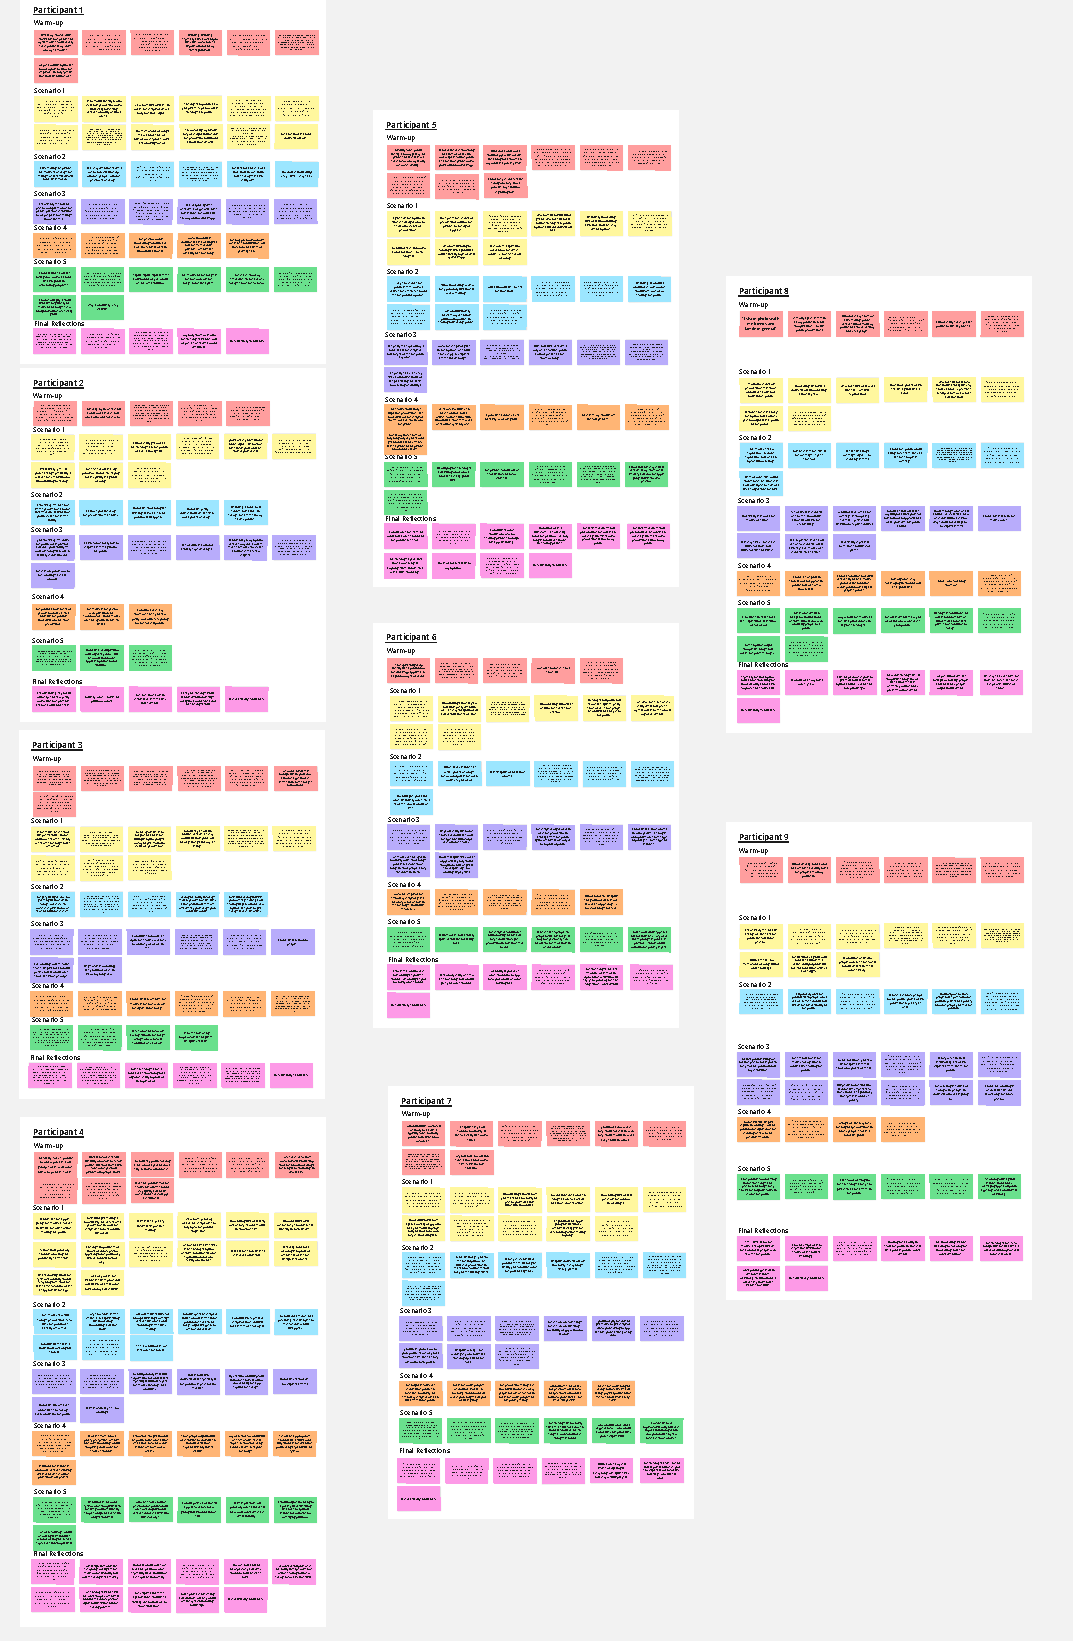
\includegraphics[page=1,width=0.75\textwidth]{appendix-materials/thematic-analysis/interview-extracts-raw-board.pdf}
\end{center}

\newpage
\section{Inductive codebook (initial iteration)}
\label{app:thematic-codebook-initial}

\noindent
First page of the initial 56-code codebook produced through close reading of the interview transcripts.

\begin{center}
  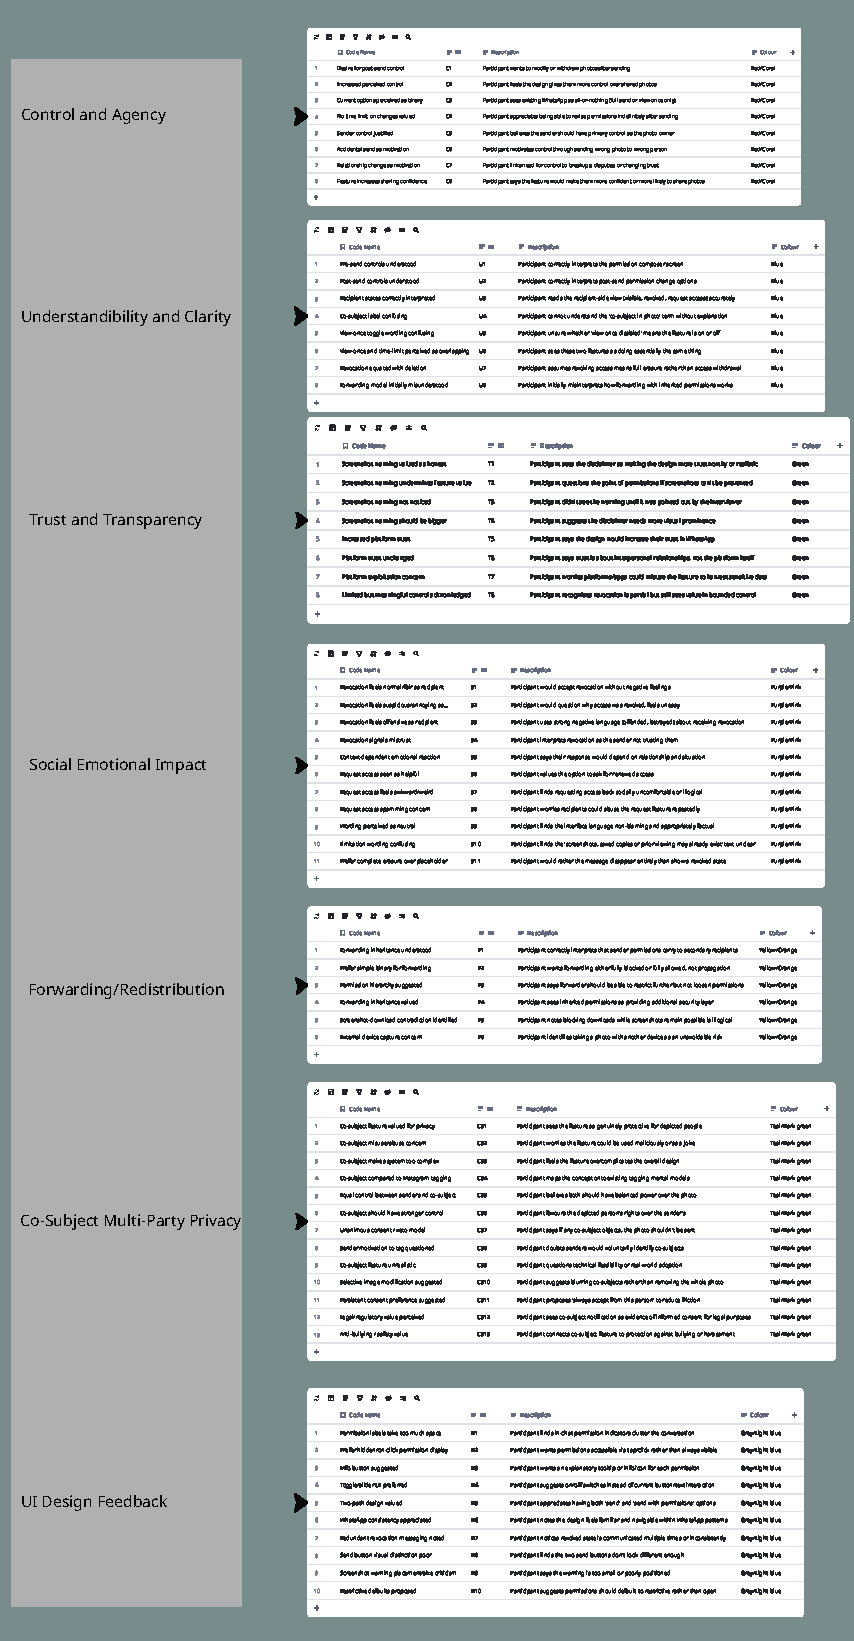
\includegraphics[page=1,width=0.75\textwidth]{appendix-materials/thematic-analysis/inductive-codebook-initial.pdf}
\end{center}


\section{Interview extracts (refined subset)}
\label{app:thematic-quotes-refined}

\noindent
First page of the refined extract set used for focused coding.

\begin{center}
  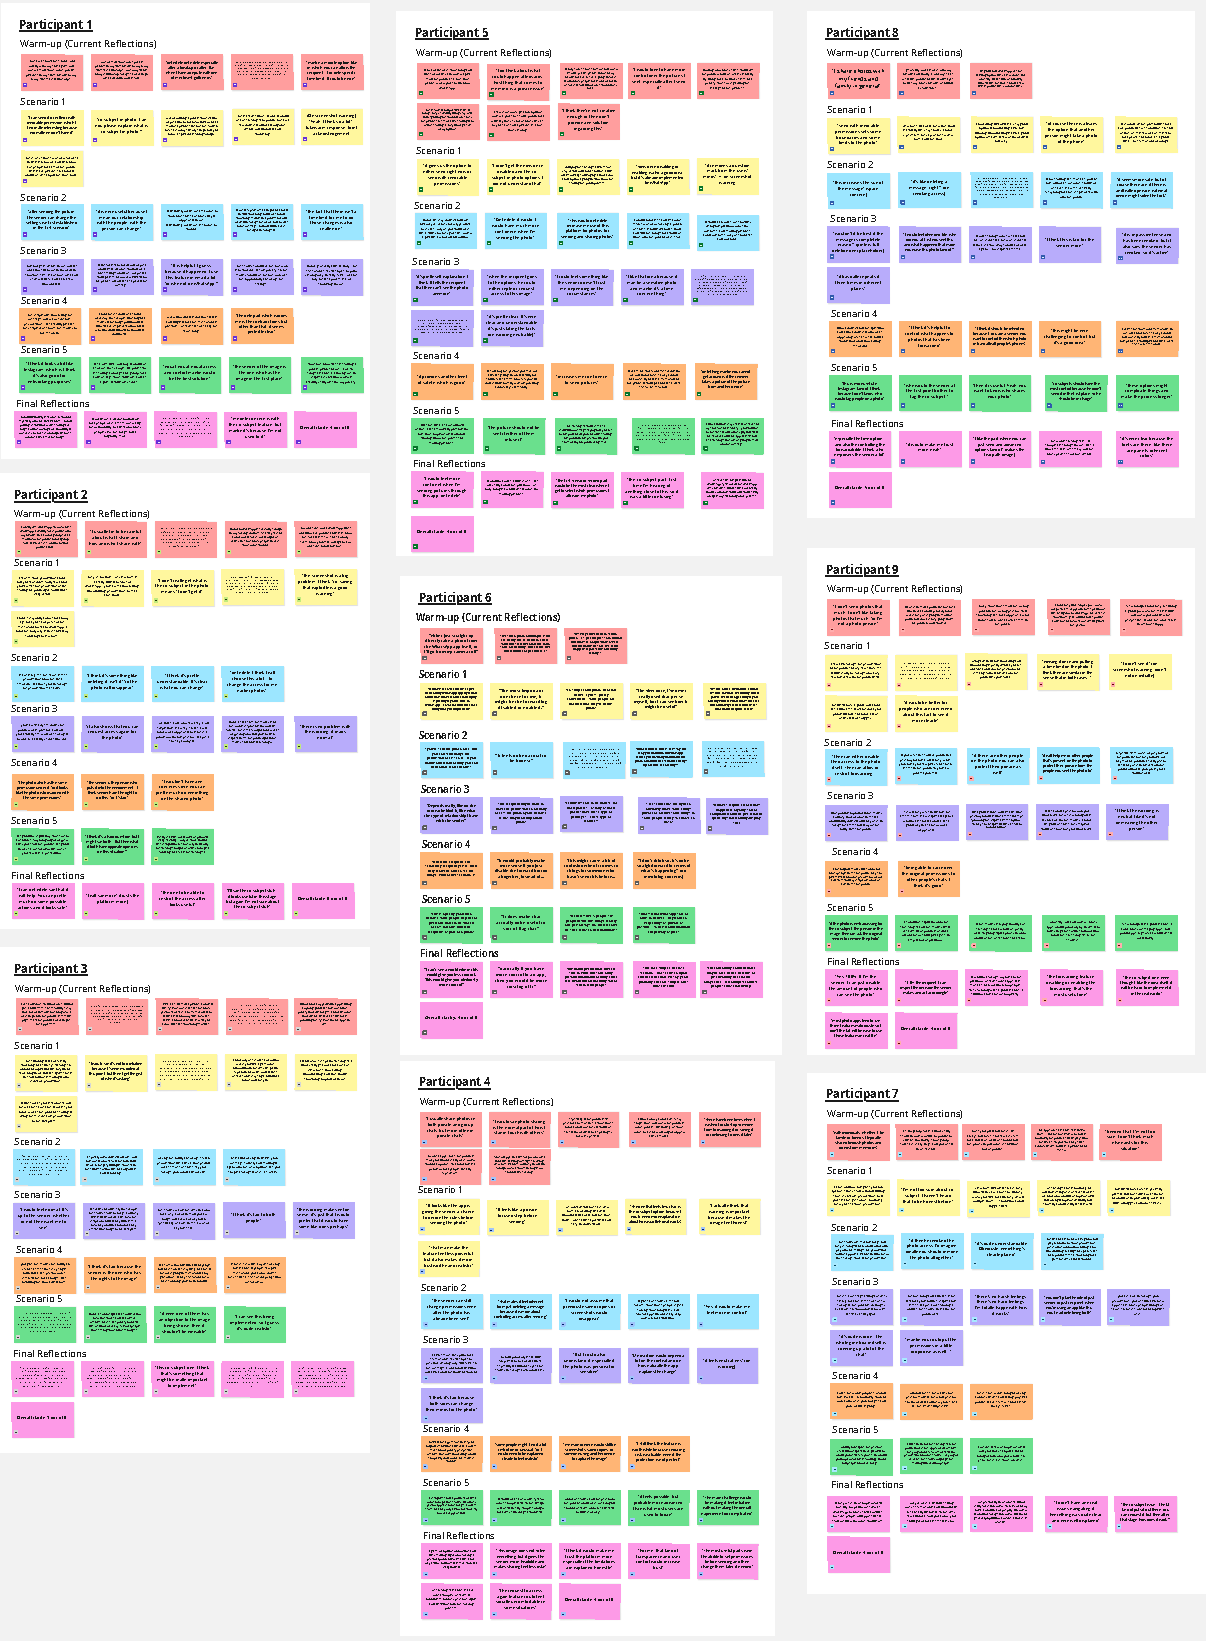
\includegraphics[page=1,width=\textwidth]{appendix-materials/thematic-analysis/interview-extracts-refined.pdf}
\end{center}

\newpage
\section{Working codebook (simplified)}
\label{app:thematic-codebook-working}

\noindent
First page of the simplified 20-code working codebook used for cross-case tagging.

\begin{center}
  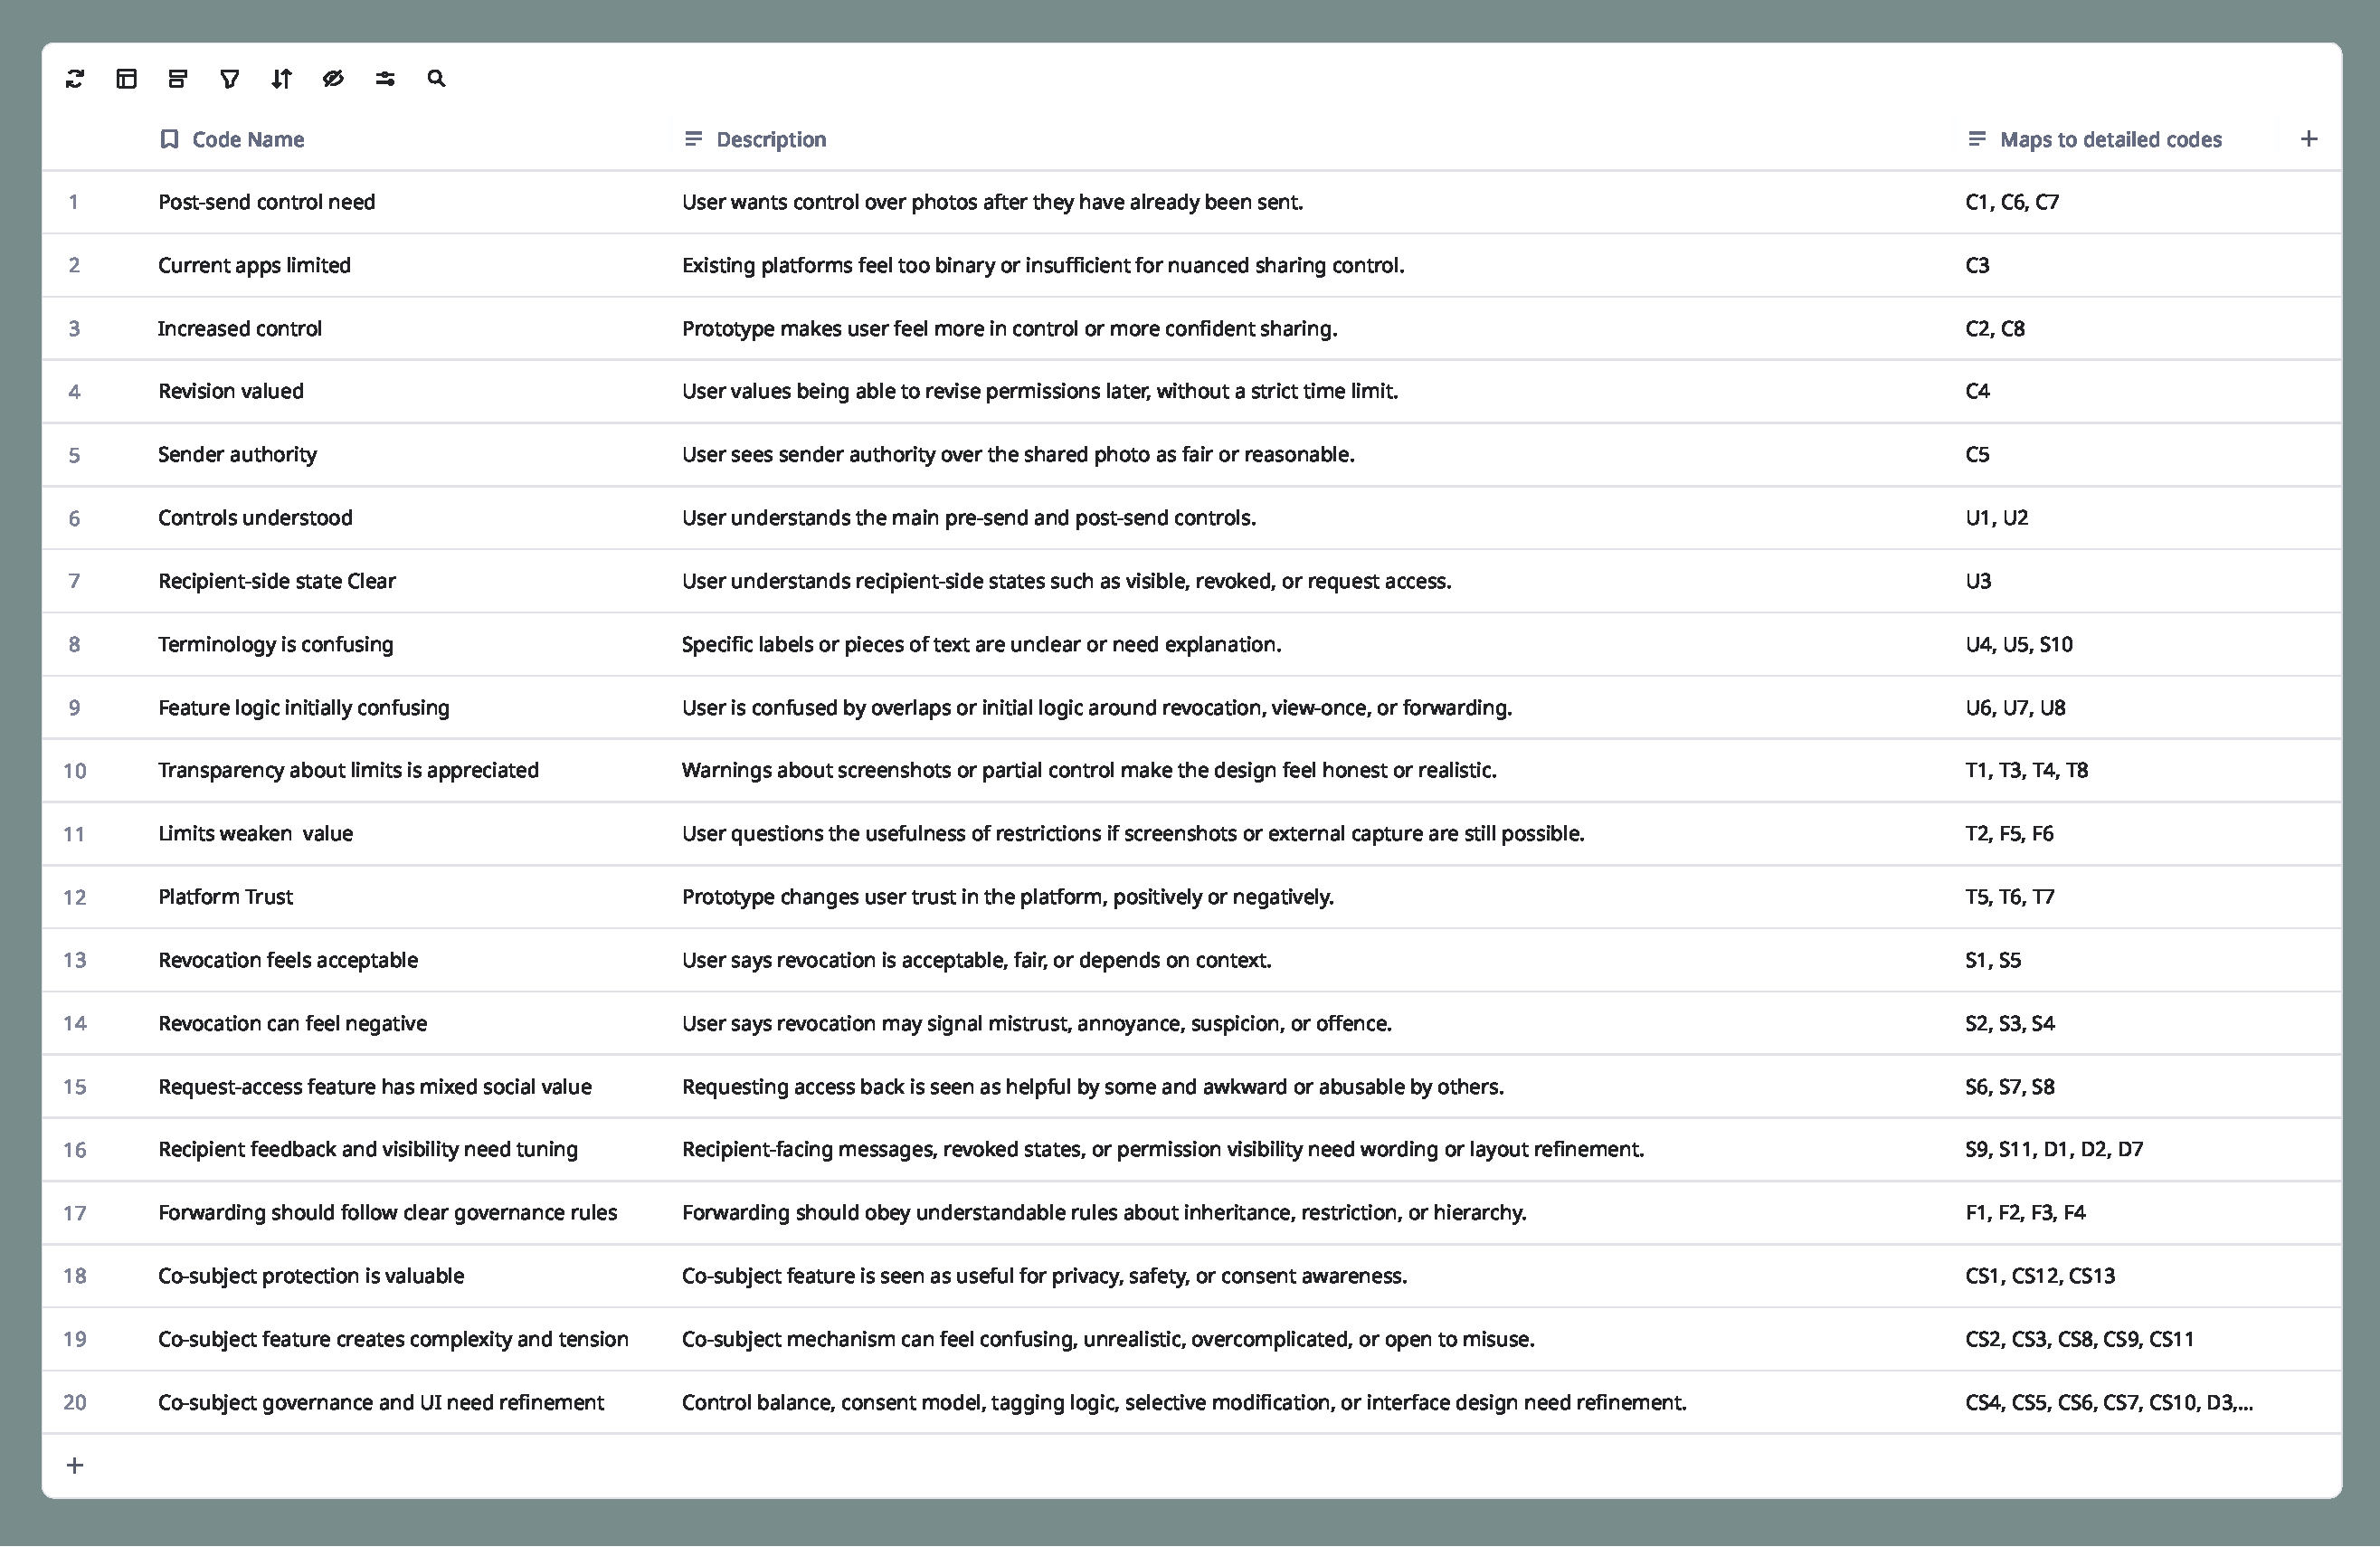
\includegraphics[page=1,width=\textwidth,height=0.88\textheight,keepaspectratio]{appendix-materials/thematic-analysis/working-codebook-simplified.pdf}
\end{center}

\newpage
\section{Quote-to-code coding sheet}
\label{app:thematic-coding-sheet}

\noindent
First page of the quote-to-code mapping sheet.

\begin{center}
  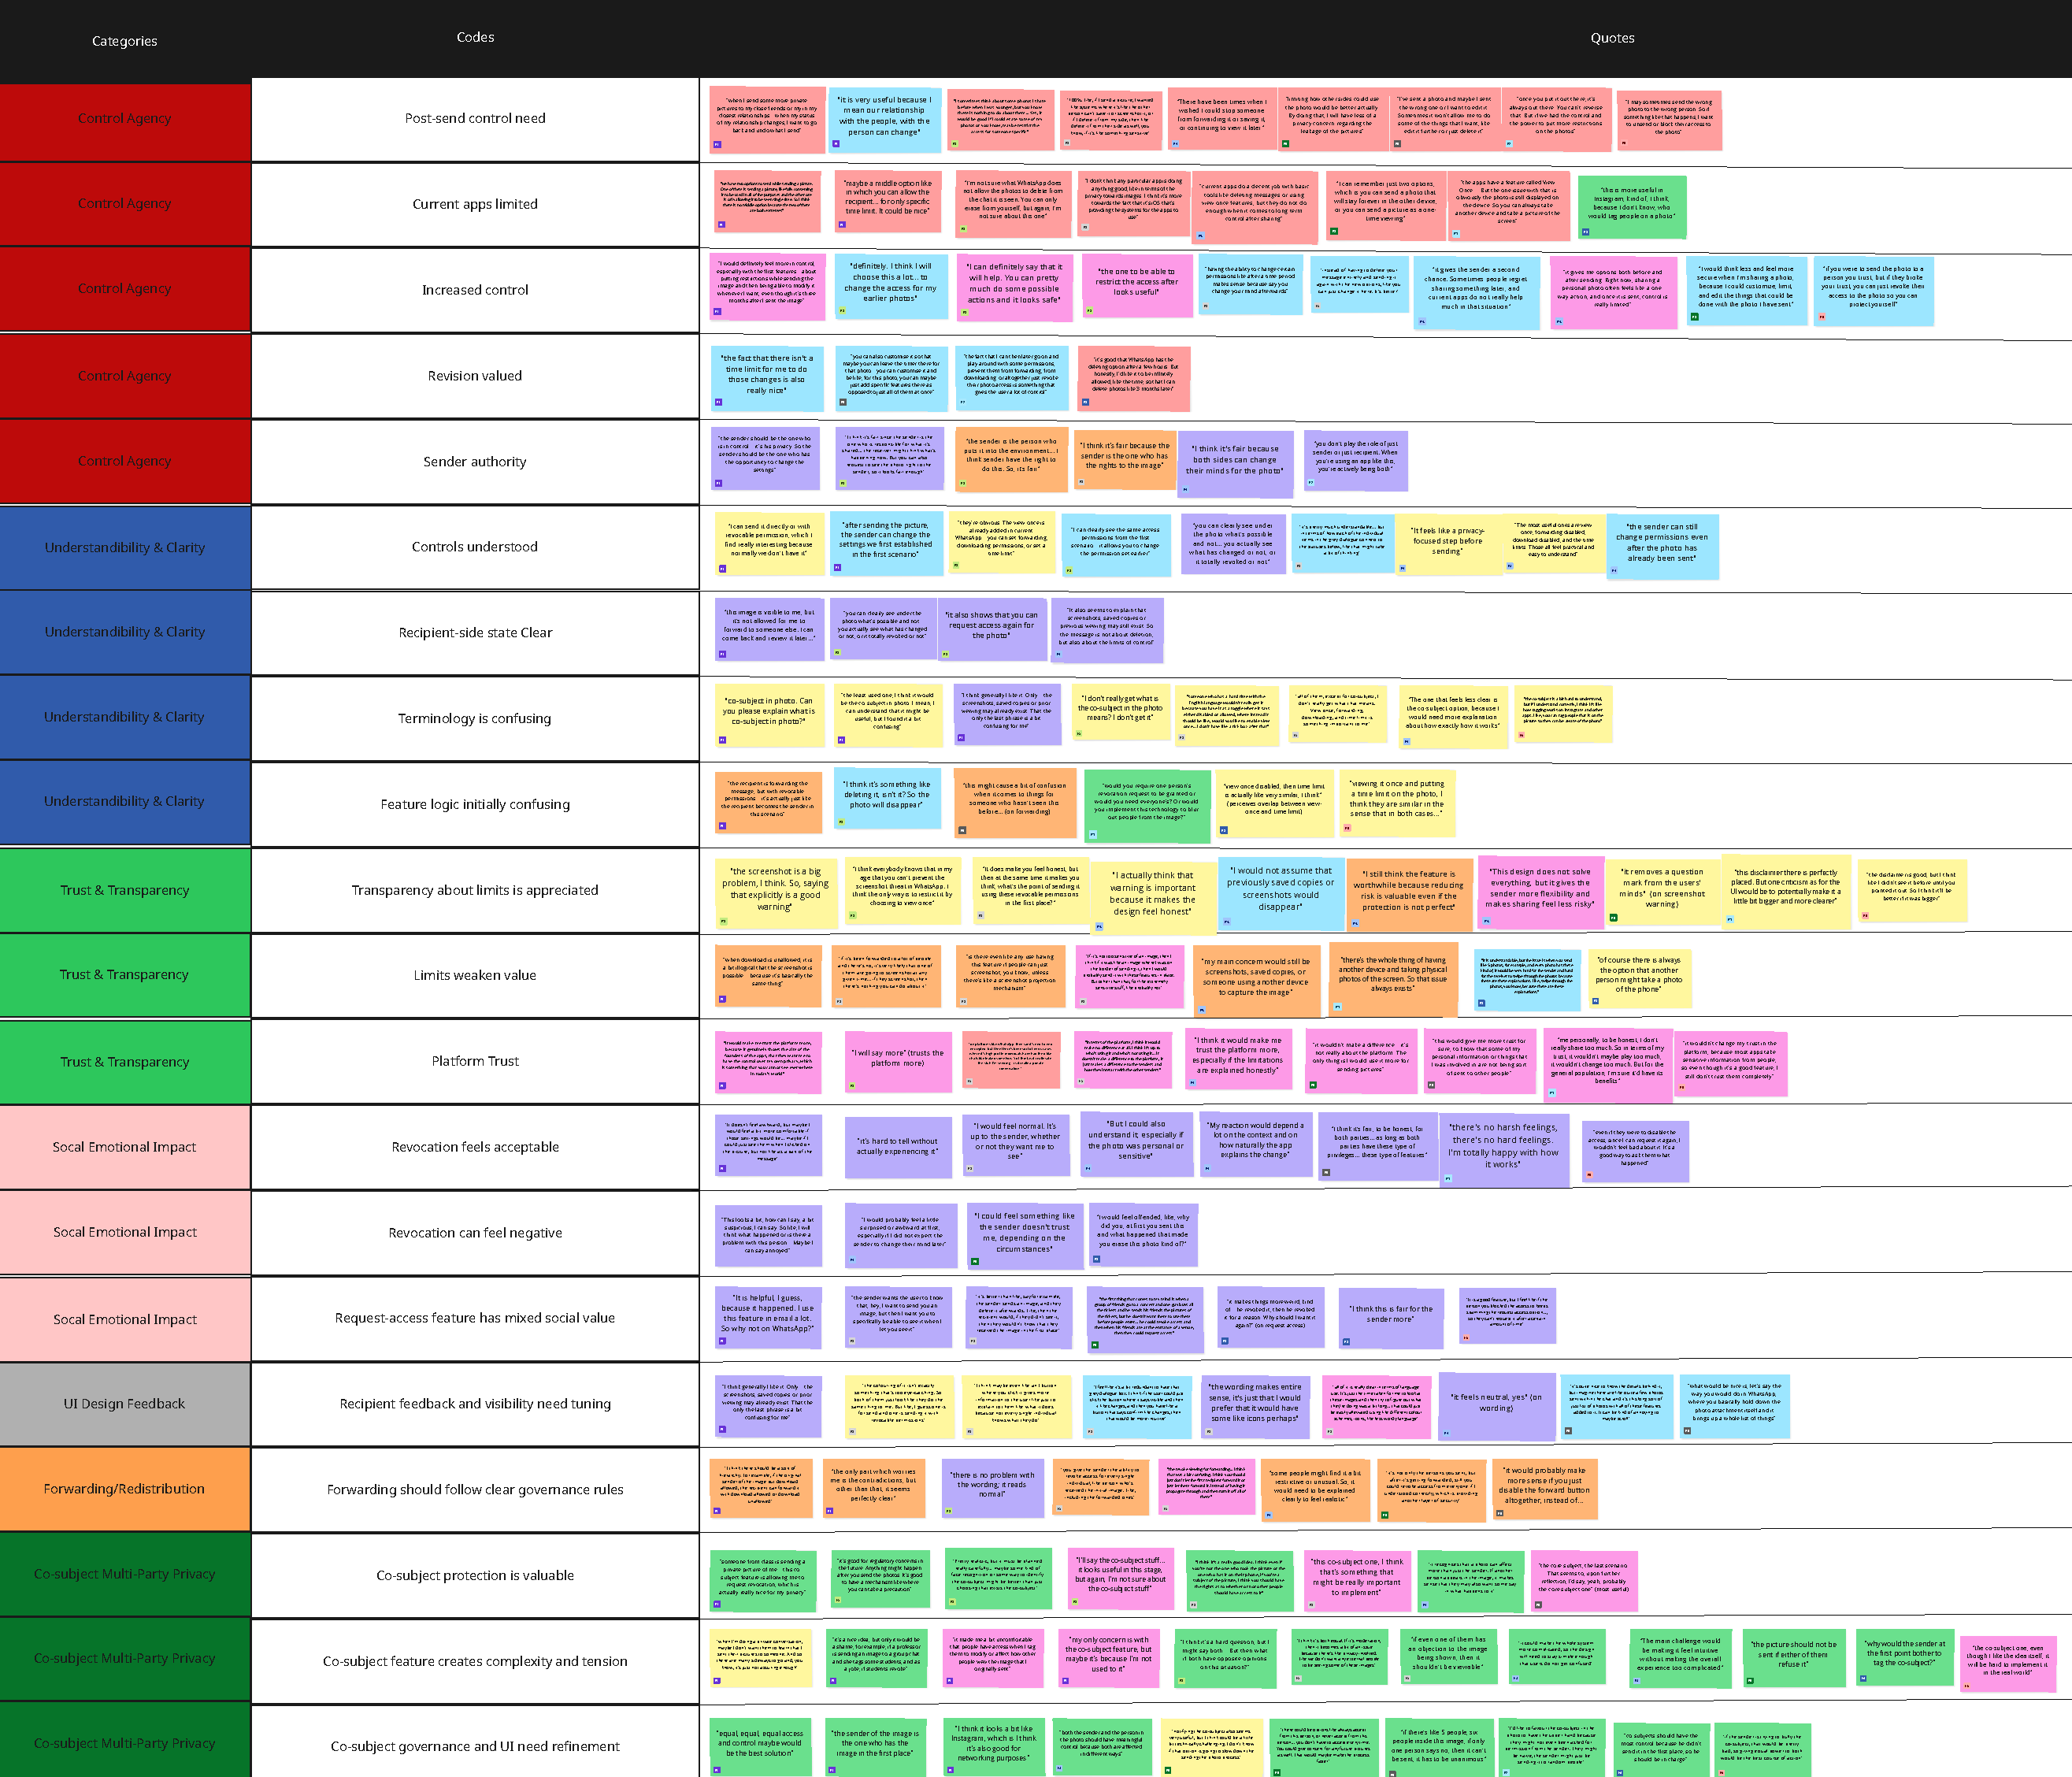
\includegraphics[page=1,width=\textwidth,height=0.88\textheight,keepaspectratio]{appendix-materials/thematic-analysis/quote-to-code-coding-sheet.pdf}
\end{center}

\newpage
\section{Final themes table}
\label{app:thematic-themes-table}

\noindent
First page of the consolidated themes table (definitions, codes, and example quotations).

\begin{center}
  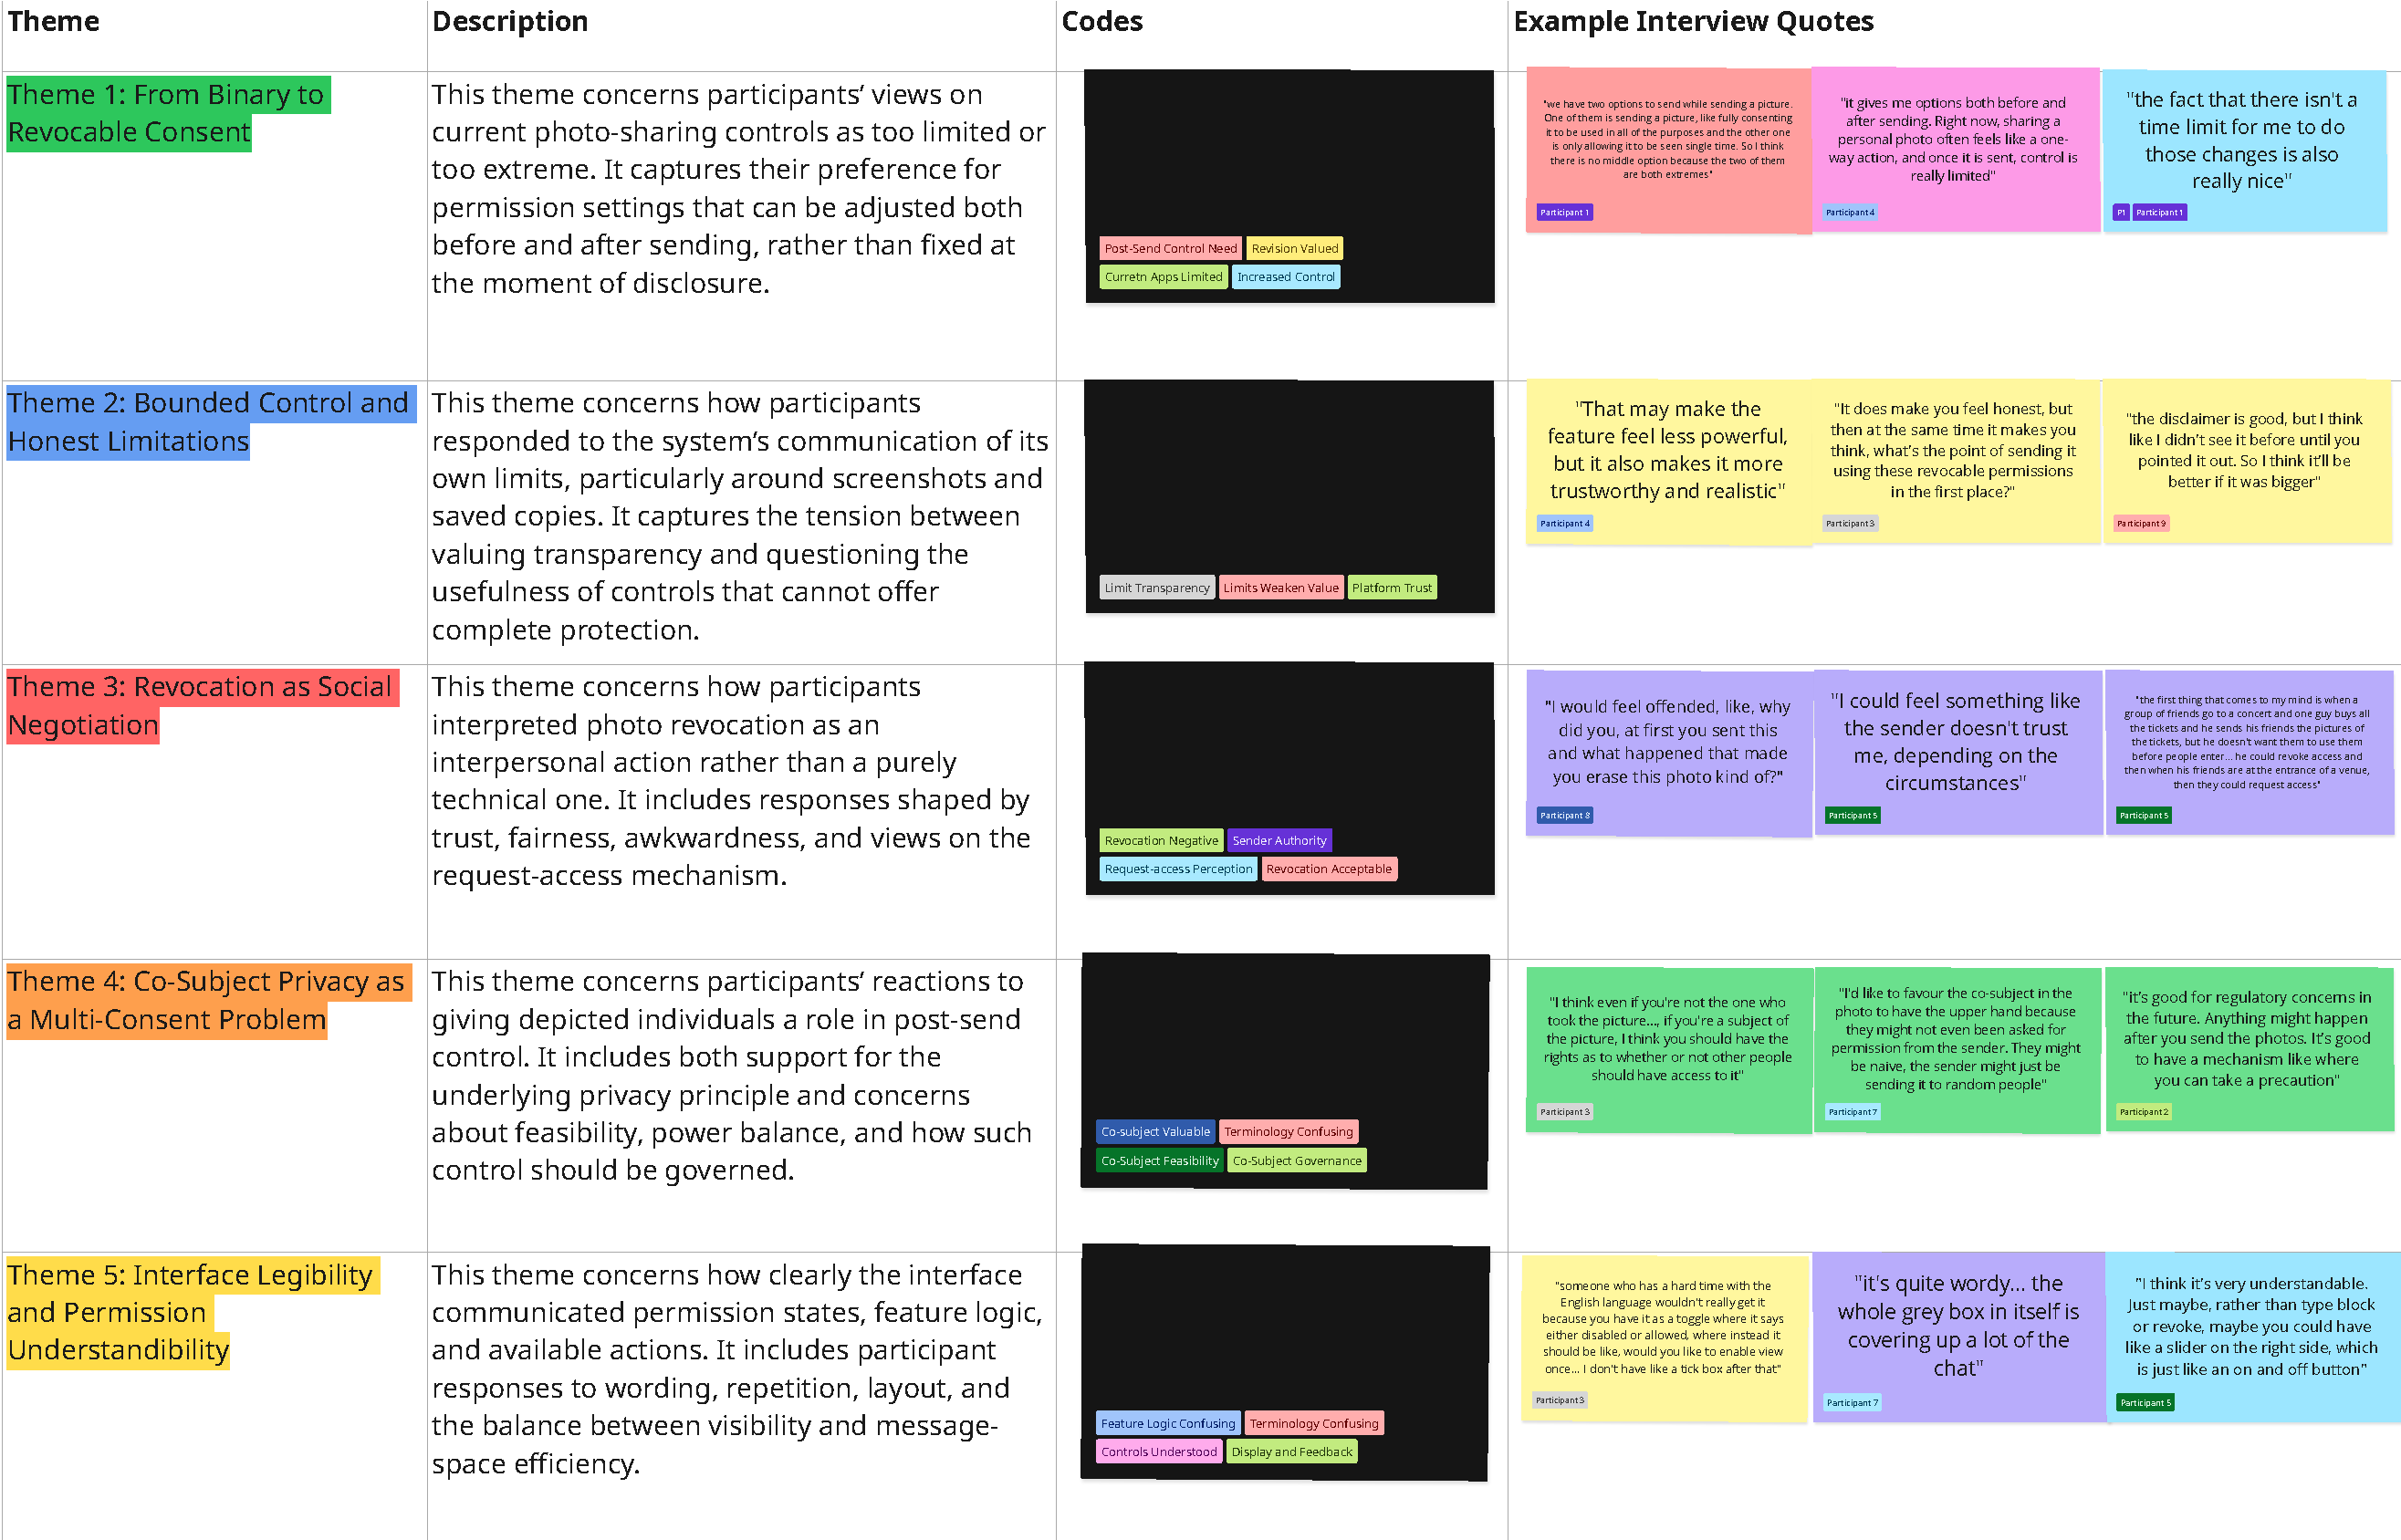
\includegraphics[page=1,width=\textwidth,height=0.88\textheight,keepaspectratio]{appendix-materials/thematic-analysis/final-themes-table.pdf}
\end{center}








\chapter{User Guide}
\label{app:user-guide}

\section{Purpose}
\label{sec:user-guide-purpose}

\noindent
 This appendix explains how to run the \textbf{Smart Photos} prototype on a local machine. Also a deployed version can be accessed at \url{https://smart-photos.vercel.app}.
A concise, illustrated tour of every major flow is already given in Section~\ref{sec:translation}. 

\section{Prerequisites}

\begin{itemize}
  \item \textbf{Node.js} version \textbf{20.x} (LTS recommended). The project uses TypeScript tooling aligned with Node~20; older major versions may fail to install or run dependencies.
  \item \textbf{npm} (bundled with Node.js). The instructions below use \texttt{npm}
\end{itemize}

\section{Install and run}

\begin{enumerate}
  \item Open a terminal and change into the prototype folder:
  \begin{verbatim}
cd photo-revocation-prototype
  \end{verbatim}
  \item Install dependencies:
  \begin{verbatim}
npm install
  \end{verbatim}
  \item Start the development server:
  \begin{verbatim}
npm run dev
  \end{verbatim}
  \item Open the default address printed in the terminal and make it full screen to have a better view. 
\end{enumerate}

\section{Optional: production build}

\noindent
To run an optimised build (closer to a deployed Next.js app, useful for a stable demo):

\begin{verbatim}
npm run build
npm run start
\end{verbatim}

\section{Feature checklist (where to see each behaviour)}


\begin{center}
\small
\begin{tabular}{@{}P{3.6cm}P{9.8cm}@{}}
\hline
\textbf{Feature} & \textbf{What to do in the running prototype} \\
\hline
Pre-send permissions and screenshot warning & From the sender handset, open the photo picker, choose one or more images, then use \emph{Send with revocable permissions}. \\
\hline
Post-send permission changes / revocation & On the sender handset, open the action menu on a sent photo message and use the post-send options (e.g.\ revoke access, forwarding, download, time limit). Expand the permission summary row under the bubble if needed. \\
\hline
Recipient view and revoked placeholder & Compare the recipient handset before and after sender-side revocation. Use recipient menu actions such as \emph{Forward}, \emph{Download}, or \emph{Request access} when the design allows them. \\
\hline
View-once consumption & On the recipient handset, open a view-once photo via \emph{Open}, then close the viewer and observe the consumed state on the bubble. \\
\hline
Forwarding and access request & Forward from a recipient handset when permitted. After revocation, use \emph{Request access} and respond on the sender handset with \emph{Accept} or \emph{Reject}. Observe the forwarded-recipient panel for propagated state. \\
\hline
Co-subject flow & Use the co-subject handset panel. Read the notification card, open the photo menu, and use \emph{Request revocation} where available. Complete \emph{Accept}/\emph{Reject} on the sender handset. \\
\hline
\end{tabular}
\end{center}

\section{Optional: automated tests}

\noindent

\begin{verbatim}
npm run test:coverage
\end{verbatim}

\noindent
Further detail on testing is given in Section~\ref{sec:software-testing}.

\chapter{Source Code}
\label{app:source-code}

\section*{Authorship statement}

\noindent
I verify that I am the sole author of the programs contained in this folder, except where explicitly stated to the contrary.

\vspace{1em}
\noindent
\textbf{Signed:} Mert Ayranci \hfill \textbf{Date:} \today

\section{Submission contents}
\label{sec:source-submission}

\noindent
The complete source code is submitted alongside this report as a separate ZIP file. This appendix is intended as a navigation aid for that archive rather than a verbatim listing. It mirrors the structure of the prototype repository and gives a one-line description of every file or unit.

The prototype is a Next.js (App~Router) front-end written in TypeScript, styled with Tailwind CSS, and tested with Vitest and React Testing Library. Build and run instructions are provided in Appendix~\ref{app:user-guide}; the architectural narrative is given in Chapter~\ref{sec:components-state}.

\section{Repository layout}
\label{sec:source-layout}

\noindent
At the top level the archive is organised as follows:

\begin{center}
\small
\begin{tabular}{@{}P{3.6cm}P{9.8cm}@{}}
\hline
\textbf{Path} & \textbf{Purpose} \\
\hline
\texttt{src/app/} & Next.js App Router entry point, root layout, and global stylesheet. \\
\texttt{src/components/photo-\linebreak[0]revocation-demo/} & React components implementing every interface region of the prototype. \\
\texttt{src/lib/photo-\linebreak[0]revocation-demo/} & Domain types, helper functions, constants, and initial in-memory state. \\
\texttt{src/lib/} & Cross-cutting permission logic shared between components and tests. \\
\texttt{tests/} & Vitest suite organised into \texttt{unit/}, \texttt{components/}, \texttt{app/}, and shared \texttt{helpers/}. \\
Root configuration & TypeScript, Next.js, Vitest, ESLint, Tailwind PostCSS, and package manifest files. \\
\hline
\end{tabular}
\end{center}

\section{File index}
\label{sec:source-index}

\noindent
The following table lists every file in the submitted archive, grouped by directory, with a one-line description of its responsibility.

\subsection*{Application entry (\texttt{src/app/})}

\begin{center}
\small
\begin{tabular}{@{}P{4.6cm}P{9.0cm}@{}}
\hline
\textbf{File} & \textbf{Description} \\
\hline
\texttt{page.tsx} & Thin route component that mounts the \texttt{PhotoRevoca\-tionDemo} orchestrator on the root URL. \\
\texttt{layout.tsx} & Root layout, metadata, and font configuration applied to every page. \\
\texttt{globals.css} & Tailwind CSS entry point and global style resets. \\
\hline
\end{tabular}
\end{center}

\subsection*{Domain logic (\texttt{src/lib/})}

\begin{center}
\small
\begin{tabular}{@{}P{4.6cm}P{9.0cm}@{}}
\hline
\textbf{File} & \textbf{Description} \\
\hline
\texttt{photoModel.ts} & Pure permission model: \texttt{computeEffectiveStatus}, \texttt{forwardingAllowed}, \texttt{formatExpiryCountdown}, and time-limit helpers. \\
\texttt{photo-revoca\-tion-demo/types.ts} & TypeScript types for messages, permissions, participants, and modal state (single source of truth for the data model). \\
\texttt{photo-revoca\-tion-demo/constants.ts} & Static configuration: scroll-wheel sizing and the preset photo album. \\
\texttt{photo-revoca\-tion-demo/initialState.ts} & Default draft permissions, default time limits, initial conversation, and send-history seeds. \\
\texttt{photo-revoca\-tion-demo/helpers.ts} & Derivation helpers used by the UI: \texttt{getEffectivePermissions}, \texttt{getSourcePolicyPermissions}, view-once consumption checks, and download utilities. \\
\hline
\end{tabular}
\end{center}

\subsection*{React components (\texttt{src/components/photo-revocation-demo/})}

\begin{center}
\small
\begin{tabular}{@{}P{5.2cm}P{8.4cm}@{}}
\hline
\textbf{File} & \textbf{Description} \\
\hline
\texttt{PhotoRevocationDemo.tsx} & Central orchestrator: owns all shared state, handlers, and the four-handset layout. \\
\texttt{PhoneFrame.tsx} & Renders the device chrome for each stakeholder view and provides the per-handset overlay context. \\
\texttt{chatPanelPortalContext.tsx} & React context exposing portal and scroll references so overlays render inside the correct handset. \\
\texttt{MessageList.tsx} & Iterates a message array and dispatches each entry to a text or photo bubble. \\
\texttt{TextMessageBubble.tsx} & Renders text, reply previews, and accept/reject controls for access and revocation requests. \\
\texttt{PhotoMessageBubble.tsx} & Renders photo messages, the collapsible permission summary, role-aware action menu, and revocation submenu. \\
\texttt{PhotoPreview.tsx} & Renders a single photo asset with placeholder, view-once, and revoked variants. \\
\texttt{PhotoStackGrid.tsx} & Multi-photo collage layout for messages with several attached assets. \\
\texttt{PhotoStackLightbox.tsx} & Full-screen gallery viewer that portals into the active handset frame. \\
\texttt{ComposerView.tsx} & Pre-send composer with caption input, permission chips, and the screenshot warning. \\
\texttt{PickerSheet.tsx} & Photo picker sheet with multi-select and the dual \emph{Send}/\emph{Send with revocable permissions} actions. \\
\texttt{ScrollWheelColumn.tsx} & Reusable wheel control used by the time-limit picker. \\
\texttt{TimeLimitModal.tsx} & Post-send modal for adjusting a photo's expiry. \\
\texttt{RequestAccessPanel.tsx} & Inline footer panel for recipients to compose an access request. \\
\texttt{RequestRevocationPanel.tsx} & Inline footer panel for co-subjects to compose a revocation request. \\
\texttt{ViewOnceInChatModal.tsx} & Full-screen viewer that handles the view-once consumption lifecycle. \\
\texttt{ViewOnceSingleTick.tsx} & Small SVG indicator marking a view-once photo as consumed. \\
\texttt{PrototypeStateSummary.tsx} & Side panel exposing the live canonical permission record for evaluator inspection. \\
\hline
\end{tabular}
\end{center}

\subsection*{Tests (\texttt{tests/})}

\noindent
File names below are listed relative to the \texttt{tests/} root and are grouped by sub-directory.

\begin{center}
\footnotesize
\begin{tabular}{@{}P{5.8cm}P{8.0cm}@{}}
\hline
\textbf{File} & \textbf{Description} \\
\hline
\texttt{unit/photoModel.test.ts} & Unit tests for the pure permission model and time-limit helpers. \\
\texttt{unit/helpers.test.ts} & Unit tests for derivation helpers, including effective-status fallbacks. \\
\texttt{components/ComposerView.\linebreak[0]test.tsx} & Component tests for the caption input, permission chips, and the warning banner. \\
\texttt{components/PickerSheet.\linebreak[0]test.tsx} & Component tests for multi-select and the two send actions. \\
\texttt{components/PhotoMessageBubble.\linebreak[0]test.tsx} & Branch tests for active, revoked, view-once, and download-disabled variants. \\
\texttt{components/PhotoStackGrid.\linebreak[0]test.tsx} & Layout tests for multi-photo collages. \\
\texttt{components/PhotoStackLightbox.\linebreak[0]test.tsx} & Tests for the portalled full-screen gallery. \\
\texttt{components/RequestPanels.\linebreak[0]test.tsx} & Tests for both inline request panels (access and revocation). \\
\texttt{components/ScrollWheelColumn.\linebreak[0]test.tsx} & Tests for the duration picker primitive. \\
\texttt{components/TimeLimitModal.\linebreak[0]test.tsx} & Tests for applying and cancelling post-send expiry changes. \\
\texttt{components/TextMessageBubble.\linebreak[0]test.tsx} & Tests for replies and request response controls. \\
\texttt{components/ViewOnceInChatModal.\linebreak[0]test.tsx} & Tests for view-once open, close, and consumption state. \\
\texttt{components/ViewOnceSingleTick.\linebreak[0]test.tsx} & Snapshot test for the consumed indicator. \\
\texttt{components/PrototypeStateSummary.\linebreak[0]test.tsx} & Tests that the state panel reflects the canonical record. \\
\texttt{components/PhotoRevocationDemo.\linebreak[0]test.tsx} & Integration-style journeys covering revocation, forwarding, and request flows across handsets. \\
\texttt{app/page.test.tsx} & Smoke test that the route mounts the orchestrator without error. \\
\texttt{helpers/photoDemoUi.tsx} & Shared Testing Library locators and assertions reused across integration tests. \\
\hline
\end{tabular}
\end{center}

\subsection*{Documentation (\texttt{docs/})}

\begin{center}
\small
\begin{tabular}{@{}P{4.6cm}P{9.0cm}@{}}
\hline
\textbf{File} & \textbf{Description} \\
\hline
\texttt{README.md} (root) & Quick-start instructions, architectural overview, and test commands. \\
\hline
\end{tabular}
\end{center}

\subsection*{Configuration (root)}

\begin{center}
\small
\begin{tabular}{@{}P{4.6cm}P{9.0cm}@{}}
\hline
\textbf{File} & \textbf{Description} \\
\hline
\texttt{package.json} & Project manifest, dependency declarations, and \texttt{npm} scripts (\texttt{dev}, \texttt{build}, \texttt{start}, \texttt{test}, \texttt{test:coverage}, \texttt{lint}). \\
\texttt{package-lock.json} & Resolved dependency lockfile for reproducible installs. \\
\texttt{tsconfig.json} & TypeScript compiler configuration including the \texttt{@/*} path alias. \\
\texttt{next.config.ts} & Next.js framework configuration. \\
\texttt{next-env.d.ts} & Auto-generated Next.js TypeScript ambient declarations. \\
\texttt{vitest.config.ts} & Vitest configuration: jsdom environment, alias resolution, and coverage settings. \\
\texttt{vitest.setup.ts} & Test setup including \texttt{@testing-library/jest-dom} matchers. \\
\hline
\end{tabular}
\end{center}

\section{Notes}
\label{sec:source-notes}

\begin{itemize}
  \item All work on the prototype stopped once the archive was uploaded to KEATS. Several copies of the submitted version are retained locally and one of these copies will be used in the project examination.
  \item The deployed demonstration at \url{https://smart-photos.vercel.app} is built from the same submitted source and is provided only as a convenience; the canonical artefact for marking is the submitted ZIP archive.
  \item No third-party code is included in the archive beyond declared \texttt{npm} dependencies, which are installed at build time from \texttt{package.json} and \texttt{package-lock.json}.
\end{itemize}

\end{document}
